%\documentclass{amsart}
%\documentclass[11pt, a4paper, two-sided,]{scrreport}
\documentclass[a4paper]{article}

% COPY PASTE

\usepackage{authblk}
\usepackage[colorlinks]{hyperref}
\hypersetup{
	citecolor=blue,
   linkcolor=red,
}

\usepackage{amsmath, amssymb, amsfonts, amsfonts, amsthm,latexsym}
\usepackage[noend]{algorithmic}
\usepackage{algorithm}
\usepackage{graphics}
\usepackage{enumerate}
\usepackage[usenames]{color}
\usepackage{mathtools}
\usepackage[normalem]{ulem}
\newtheorem{theorem}{Theorem}[section]
\newtheorem{proposition}[theorem]{Proposition}%[section]
\newtheorem{lemma}[theorem]{Lemma}%[section]
\newtheorem{definition}{Definition}[section]
\newtheorem{corollary}[theorem]{Corollary}%[section]
\newtheorem{remark}[theorem]{Remark}%[section]
\newtheorem{problem}{Problem}[section]
\newtheorem{observ}{Observation}
\usepackage{url}
\RequirePackage{hyperref}
\DeclareMathOperator{\sgn}{sgn}

\DeclareSymbolFont{yhlargesymbols}{OMX}{yhex}{m}{n}
\DeclareMathAccent{\overarc}{\mathord}{yhlargesymbols}{"F3}

%%%%% SOME LOW LEVEL STUFF NEEDED FOR SPECIAL SYMBOLS 
\makeatletter
\def\moverlay{\mathpalette\mov@rlay}
\def\mov@rlay#1#2{\leavevmode\vtop{%
    \baselineskip\z@skip \lineskiplimit-\maxdimen
    \ialign{\hfil$\m@th#1##$\hfil\cr#2\crcr}}}
\newcommand{\charfusion}[3][\mathord]{
  #1{\ifx#1\mathop\vphantom{#2}\fi
    \mathpalette\mov@rlay{#2\cr#3}
  }
  \ifx#1\mathop\expandafter\displaylimits\fi}
\DeclareRobustCommand\bigop[1]{%
  \mathop{\vphantom{\sum}\mathpalette\bigop@{#1}}\slimits@
}
\newcommand{\bigop@}[2]{%
  \vcenter{%
    \sbox\z@{$#1\sum$}%
    \hbox{\resizebox{\ifx#1\displaystyle.9\fi\dimexpr\ht\z@+\dp\z@}{!}{$\m@th#2$}}%
  }%
}
\makeatother
%%%%% END LOWLEVEL USER DEFINITION 
\newcommand{\bigjoin}{\bigop{\triangledown}}
\DeclareMathOperator{\join}{\triangledown}
\newcommand{\cupdot}{\charfusion[\mathbin]{\cup}{\cdot}}
\DeclareMathOperator{\bigcupdot}{\charfusion[\mathop]{\bigcup}{\cdot}}
\definecolor{jade}{rgb}{0.0, 0.66, 0.42}
\newcommand{\child}{\mathsf{child}}
\DeclareMathOperator*{\argmax}{arg\,max}
\newcommand{\Pmax}{\mathrm{Pmax}}
\newcommand{\T}{\widetilde{T}}
\renewcommand{\t}{\widetilde{t}}
\newcommand{\AX}[1]{\textnormal{#1}}
\providecommand{\keywords}[1]{\textbf{\textit{Keywords: }} #1}
 % END COPY PASTE


\usepackage[backend=bibtex]{biblatex}
\usepackage{todonotes}
\usepackage{subcaption}
\usepackage{placeins}
\addbibresource{References.bib}

\newcommand{\algorithmicbreak}{\textbf{break}}
\newcommand{\BREAK}{\STATE \algorithmicbreak}
\newcommand{\algorithmautorefname}{Algorithm}

\author{Emanuel Berggren}
\title{Graph coloring using modular decomposition}
%template

\usepackage[T1]{fontenc}
\usepackage[utf8]{inputenc}
\usepackage{eso-pic}
\usepackage{graphicx}
\renewcommand{\familydefault}{\sfdefault}
\setlength{\parindent}{0pt}
\pagestyle{empty}
%\setlength{\headsep}{5cm}
%\setlength{\oddsidemargin}{5mm}

\newcommand{\Framsida}{\AddToShipoutPicture*{\put(0,0){\includegraphics{kandidatfram.pdf}}}}

\newcommand{\Baksida}{\AddToShipoutPicture*{\put(0,0){\includegraphics{kandidatbak.pdf}}}}
%template


\usepackage{datetime}
\newdateformat{monthyeardate}{%
      \monthname[\THEMONTH], \THEYEAR}

%
%\begin{document}
%\maketitle

\begin{document}

\Framsida 
\vspace*{4cm}
\Huge{Graph coloring using modular decomposition}\\\\ %Fyll i titel
\Large{Emanuel Berggren} %Fyll i författare

\vspace*{12cm}
\Large{Handledare: Marc Hellmuth} \\ 
\Large{Examinator: Marc Hellmuth} \\ 
\Large{Inlämningsdatum: \today}\\

%\section{Abstract}
\begin{center}
	\textbf{Abstract}
\end{center}
\textit{
Graph coloring is one of the most common and studied problems in computer
science. It has application in many different areas, such as (EXAMPLES), but
being NP-Hard means that optimal solutions are infeasible, and in turn that most
practical problems require the use of heuristics. This thesis examines a
heuristic based on the modular decomposition of a graph, a way to split the graph
into distinct partitions of vertices where some parts can be colored optimally,
and some parts require other heuristics. This strategy of coloring with the
modular decomposition was found to give an increase in performance for the
TabuCol heuristic, but no increase for the other tested heuristics.
}

%but the modular decomposition could have applicability in
%designing parallel coloring algorithms or to improve execution time with a
%practical linear time modular decomposition algorithm.



\tableofcontents

\section{Introduction}

\todo[inline]{Rewrite}

In this thesis, we investigate a new heuristic for coloring graphs using the
modular decomposition of a graph, that is used alongside other traditional
graph coloring heuristics.

The modular decomposition of a graph describes the structure of the graph, by
recursively splitting it into distinct modules. A module is a set of vertices
in a graph, which share a common neighbourhood of vertices among vertices
outside of the module. Modules also form a hierarchy, which means that modules
can be further subdivided into smaller modules. This representation of a graph
can be described with a rooted tree, where every vertex has one of three
possible labels describing how it's child modules can be combined to form the
graph induced by it's parent module. There are 3 specific types of modules,
series, parallel, and prime, which are defined later.

Modular decomposition allows for coloring of graphs in linear time with optimal
chromatic number if all of the modules are either  series or parallel
\cite{HCL}. However, if any of the vertices are prime then optimal graph
coloring is in general NP-Hard\cite{NPHard}. The question examined here, is if
one can still utilize the modular decomposition, where graph coloring heuristics
are only applied on the prime modules. The modular decomposition might still color some parts
of the graph optimally, and the structure it provides might provide a hint for
how to apply the heuristics on the prime parts, improving performance for other
heuristics.

%kanske rätt onödigt?
In \autoref{sec:Definitions} all of the required terminology and definitions are
provided, and is split into two parts, \autoref{sec:GraphBasics} has definitions that might be
familiar to most people that have worked with graphs, and
\autoref{sec:GraphModules} provide the definitions that are more specific to
this thesis.

In \autoref{sec:Heuristics} the graph coloring heuristics used are described.

In \autoref{sec:Strategies} the combination strategies are described, that is how are
these heuristics applied, and how is the structure of the modular decomposition
utilised.

In \autoref{sec:Data} the test graphs and benchmarking methods are described. The data
used is both from standard DIMACS benchmarks \cite{DIMACS}, and custom generated data.

Finally, the way the data is evaluated and the results are presented in 
\autoref{sec:Evaluation}, respectively \autoref{sec:Result}

\section{Definitions}
\label{sec:Definitions}

\subsection{Graph basics}
\label{sec:GraphBasics}

The definitions used here are based of the definitions in \cite{GraphBasics}. 
%If not stated differently, the definitions here have been taken from 
%\cite{GraphBasics}.

\begin{definition}[Graph]
    A graph $G = (V,E)$ is a tuple, where $V$ is the set of vertices, and $E$ is
    a set of unordered pairs of distinct vertices.
\end{definition}
\begin{definition}[Neighbour]
    For a graph $G = (V,E)$, we say that $v \in V$ is adjacent to 
    $u \in V$ if $(v,u) \in E$. 

    The neighbourhood $N_G(v)$ for a vertex $v \in V$ in a graph $G = (V,E)$,
    is the set of vertices that are adjacent to $v$, that is 
    $N_G(v) = \{u : (u,v) \in E \}$. If $u \in N_G(v)$, we also say
    that $u$ and $v$ are neighbours.
\end{definition}
\begin{definition}[Degree]
    The degree for a vertex $v \in V$ in a graph $G = (V,E)$, denoted by 
    $deg(v)$, is the number of neighbours for $v$ in $G$, that is 
    $deg(v) = |N_G(v)|$.
\end{definition}

In many cases, one is interested in some parts of the graph, and one of the
most common ways to decompose a graph is through the induced subgraph. An induced
subgraph is a graph constructed by only including a subset of the original
graphs vertices, and all edges between these vertices in the original graph.

\begin{definition}[Subgraph]
    A subgraph $S = (V',E')$ of a graph $G = (V,E)$, is a graph such that
    $V' \subseteq V$, $E' \subseteq E$.
\end{definition}

\begin{definition}[Induced subgraph]
    
    For a graph $G = (V,E)$, the induced subgraph $G[X]$ for $X \subseteq V$, is
    the subgraph $(X,\{(u,v) : (u,v) \in E, u \in X,v \in X\})$. 
    %That
    %is, a graph only containing the vertices in $X$, and all edges between
    %these vertices that were in the original graph.

\end{definition}

Another common operation, is the graph complement. The graph complement of a
graph is graph that contains the same vertices as the original graph, but the
vertices are adjacent only if they where not adjacent in the original graph.
This also means that the union of their edge sets contains all possible edges
between the vertices.

\begin{definition}[Graph complement]
    The graph compliment $\overline{G}$ of a graph $G = (V,E)$ is the graph 
    $(V,\{ (u,v) : u \neq v, u \in V,v \in V, (u,v) \notin E \})$.
\end{definition}

Two common operations, and especially relevant for the modular decomposition
further down, is the disjoint union and graph join. The disjoint union is the
most simple way to combine graphs, and just forms a new graph that just
contains the original graphs and nothing more.  The graph join is similar, in
that it produces a new graph with all of edges and vertices from the original
graphs, but also for every vertex in a input graph adds a new edge to the other
input graphs.

\begin{definition}[Disjoint union]
    The disjoint union $\bigcup_i G_i$ for graphs 
    $(V_1,E_1) \cdots (V_k,E_k)$ where 
    $\bigcap V_i = \varnothing $ , is the graph
    $G = \left( \bigcup V_i,\bigcup E_i \right)$.
\end{definition}

\todo[noline]{Haven't found a paper actually defining the Graph join}
\begin{definition}[Graph join]
    The graph join $\nabla G_i$ for graphs $(V_1,E_1) \cdots (V_k,E_k)$ where 
    $\bigcap_i V_i = \varnothing$, is the graph $G = (\{\bigcup V_i,
    \bigcup E_i \cup \{(u,v) : u \in V_k, v \in V_j, k \neq j \})$
\end{definition}

\todo[noline]{Fix description of connected component}

One of the original applications of graph theory was to describe different ways
to walk in city (REFERENS?), so the concept of a path has been central for a long
time.  A path is a sequence vertices, so that the next vertex in the sequence is
connected to the previous by an edge, and so that vertices are not repeated.
One can then imagine "walking" between vertices by moving on edges.

\begin{definition}[Path]
    A path $p$ in graph $G = (V,E)$ is a sequence of vertices $p = (v_1\cdots
    v_i)$, such that $(v_j,v_{j+1}) \in E$ for $1 \leq j \leq i-1$ and $v_j \neq v_k$ 
    for $0 \leq j,k \leq i-1$ when $j \neq k$.
\end{definition}

\begin{definition}[Connected graph]
    A graph $G = (V,E)$ is connected, if there exists a path between any two
    vertices in the graph. Otherwise, we say that a graph is disconnected.
\end{definition}

The central problem in this thesis, is the efficient coloring of a graph.
Coloring graph means that one assigns to every vertex a color, an arbitrary
value, such that no vertices that are neighbours have the same color. A classic
example of this problem is when coloring a map and wants to avoid giving
neighbouring countries the same color.  Every country can be represented by a
vertex, and edges are added if two countries share a border.

\begin{definition}[Graph coloring]
    A graph coloring $\sigma$ for a graph $G = (V,E)$ is a map from $V$ to $C$,
    where $C$ is a set of colors, such that no neighbours share the same color,
    that is $(u,v) \in E$ implies that $\sigma(u) \neq \sigma(v)$. We say that $\sigma$
    is a $k$ coloring if $|C| \leq k$. A graph coloring is also called a proper coloring,
    to distinguish it from a Partial coloring and an improper coloring.
\end{definition}
\begin{definition}[Partial coloring]{\cite{Constructive}}
    A partial graph coloring $\sigma$ for a graph $G = (V,E)$ is a map from $P \subset V$ to $C$,
    where $C$ is a set of colors, such that for every vertex in $P$ no neighbours 
    share the same color, that is $u \in P,v \in P, (u,v) \in E$  implies that $\sigma(u) \neq \sigma(v)$.
\end{definition}
\begin{definition}[Improper coloring]{\cite{Constructive}}
    An improper graph coloring $\sigma$ for a graph $G = (V,E)$ is a map from
    $V$ to $C$, where $C$ is a set of colors, allowing for clashes in coloring,
    that is neighbours can share the same color.
\end{definition}
\begin{definition}[Chromatic number]
    The chromatic number of a graph $G = (V,E)$, denoted by $\chi(G)$, is the
    least amount of colors needed to color the graph with a proper coloring.
\end{definition}

Finding a coloring for a graph is easy, one could for example 
assign every vertex a unique color. Finding an optimal coloring however, a coloring using the
fewest possible colors, is NP-Hard \cite{NPHard}. For this purpose, multiple
different heuristics, algorithms providing a proper coloring with as few colors
as possible but not necessarily optimal, have to be used.

\begin{definition}[Complete graph]
    A graph $K = (V,E)$ is complete if every vertex in $v \in V$ is adjacent to
    every other vertex, that is, $ (u,v) \in E \iff v \neq u$. We also call the
    graph $K_n$ with the complete graph that has $n$ vertices.
\end{definition}

\subsection{Graph modules and cographs}
\label{sec:GraphModules}

\begin{definition}[Cograph]{\cite{CoGraph}}
  A graph $G$ is a \emph{cograph} if $G=K_1$, $G$ is the disjoint union
  $G=\bigcupdot_i G_i$ of cographs $G_i$, or $G$ is a join
  $G=\bigjoin_i G_i$ of cographs $G_i$.
\end{definition}


\begin{definition}[Graph module]{\cite{Module}}
    Let $G = (V,E)$ be an arbitrary graph. A non-empty vertex set $M \subseteq V$
    is a module of $G$ if, $\forall x,y \in M (N_G(x) \setminus M = N_G(y) \setminus M)  $. A module $M$ is
    strong if it does not overlap with any other module $M'$, i.e, if 
    $M \cap M' \in \{M,M',\emptyset \}$.
\end{definition}
  

Now we have sufficient terminology to describe the most central concept, the
modular decomposition. The modular decomposition is way to partition the
vertices of the graph into a tree structure, where the relation between
different modules, parts in the partitions, are known. Another way to look at
the modular decomposition, is that it's a cograph approximation of the original
graph, where parts that don't have a cograph structure are replaced with prime
modules.

\todo[noline]{Update definition. Unsure which paper to cite}
\begin{definition}[Modular decomposition]{\cite{HCL}}
    The modular decomposition MD for a graph $G =(V,E)$, is the set of all
    strong modules of the graph.
\end{definition}

The modular decomposition of a graph has a number of useful properties. The
modular decomposition of a graph forms a hierarchy (REFERENS), meaning that strong modules
can be partitioned into other strong modules. This hierarchy of modules has a
natural representation as a tree, the modular decomposition tree.

This tree describes the structure of the modular decomposition of the original
graph. Every vertex in the tree represents a strong module, with the root being
the strong module containing all vertices. This tree also describes how the
induced subgraph of the module can be constructed from the induced subgraphs of
it's children.

\todo[noline]{What could be a proper reference...}
\begin{definition}[Modular decomposition tree]{\cite{HCL}}
    The modular decomposition tree $(\T,\t)$ of a graph $G = (V,E)$,is a rooted
    vertex labeled tree such that every vertex is associated with a strong
    module $X$ in $G$, and with a label distinguishing 3 cases.
    \begin{enumerate}
        \item Series: $G[X]$ is disconnected.
        \item Parallel: $\overline{G[X]}$ is disconnected.
        \item Prime: $G[X]$ and $\overline{G[X]}$ is disconnected.
    \end{enumerate}
    And such that the root of the tree has $V$ as the associated vertex, and all 
    strong modules are a part of the tree.
\end{definition}

Note, a label being series in modular decomposition tree with associated module
$X$ means that the induced subgraph $G[X]$ can be constructed through graph
union on the induced subgraphs of its children's associated modules, and it being
parallel means that $G[X]$ can be constructed through graph join on the
induced subgraphs of its childrens associated modules \cite{HCL}.

As a single vertex is a module, every leaf of the modular decomposition has
a single vertex as a module. This means that a modular decomposition without
prime modules is a cograph, as it is recursively constructed by graph join and
graph union on $K_1$.

The modular decomposition of a graph and its corresponding modular
decomposition tree is unique \cite{MDUnique}, which means that the construction
of the modular decomposition doesn't vary and need not be a part of
the heuristic.


\section{General coloring algorithm}

The algorithm used for coloring is \autoref{alg:generic}, described in
\cite{HCL}. It provides an optimal coloring given that the graph is a cograph,
that is when all modules in the modular decomposition tree is either series or
parallel.  It does however not provide a way to color the prime modules. This
paper examines multiple different ways these prime modules can be colored, split
into 2 parts, a heuristic used, and a coloring strategy. 

\autoref{alg:generic} starts by first assigning every vertex a unique color,
and then colors the modules recursively, starting at the root. The children of a
module is colored before module itself is colored. How a module is colored depends 
on which type it is, series, parallel, and prime.

A module $X$ being series in the modular decomposition tree of a graph $G$
means, as stated earlier, that the induced subgraph $G[X]$ can be
constructed through graph join on the induced subgraph of $X's$ children in the
modular decomposition. This means that every child module is completely
connected to the other children, most importantly meaning that no child modules
can share a color among the other child modules. Assuming that the children
have an optimal coloring, their join therefore also has an optimal coloring, as
no fewer colors can be used. Having initially given every vertex a unique
color, we can also guarantee that this join won't introduce any clashes. This
case is therefore "omitted" from the algorithm, as doing nothing, keeping the
current coloring, is all that needs to be done.

A module being $X$ series in the modular decomposition tree of a graph $G$ means that
the induced subgraph $G[X]$ can be constructed through disjoint union on the induced
subgraph of the associated modules of $X's$ children. This in particular means that 
the induced subgraph of the children modules have no edges between each other. Therefore,
the induced subgraph of the children modules can use the same set of colors. The children
are therefore recolored with the minimum amount of colors needed, 
which assuming that the children are optimally colored is the amount of colors used by the module 
with the most amount of colors.

The last case is when the module is prime. Coloring this module is in the
general case NP-Hard. This paper examines how this prime module can be colored,
replacing line 12 with a graph coloring heuristic. The question is whether or
not the performance is improved when applying this heuristic locally on these
prime module compared to applying this heuristic on the whole graph.

\begin{algorithm}[H]
  \caption{Modularly-minimal coloring a graph $G$ with MD tree $(T,t)$.}
  \label{alg:generic}
  \algsetup{linenodelimiter=}
  \begin{algorithmic}[1]
    \REQUIRE Graph $G$ and MD tree $(\T,\t)$
    \STATE Initialize a coloring $\sigma$ s.t.\ all $v \in V(G)$
           have different colors
      \FORALL{$u\in V^{0}(T)$ \text{in post order}}
       \IF {$u$ is parallel} 
          \STATE $\mathcal{G} \leftarrow \{G(w)\colon w\in\child(u)\}$ 
          \STATE $G^* \leftarrow \argmax_{w\in\child(v)} |\chi(G(w))|$
          \STATE $S \leftarrow \sigma(V(G^*))$ 
          \FOR {$H\in\mathcal{G}\setminus \{G^*\}$} 
             \STATE randomly choose an injective map $\phi:\sigma(H)\to S$
             \FORALL {$x\in H$}
                \STATE $\sigma(x)\leftarrow \phi(\sigma(x))$  
             \ENDFOR
          \ENDFOR
       \ELSIF{$u$ is \emph{prime}} 
          \STATE Construct a modularly-minimal coloring of $G(u)$
              with colors contained in $\sigma(G(u))$
              and adjust $\sigma$ accordingly 
       \ENDIF
    \ENDFOR
  \end{algorithmic}
\end{algorithm}

\autoref{alg:generic} is therefore used in combination with a graph coloring
heuristic. The heuristics tested in combination with \autoref{alg:generic} is
described below, in \autoref{sec:Heuristics}.

To distinguish the different ways the graph is colored, a strategy is also
defined below, in \autoref{sec:Strategies}.  The strategy describes how the
heuristic is used, and two have already been described here, applying it locally
on the prime modules, or applying it on the whole graph, not utilising the
modular decomposition at all. Every way a graph is colored here can therefore be
described by specifying which heuristic which strategy is used.

\section{Heuristics}
\label{sec:Heuristics}

%ska man ta med sånt alla vet
A graph coloring heuristic is an algorithm for coloring a graph, that doesn't
necessarily give an optimal coloring, but uses various methods to approximate a
good coloring.


In this section, the different heuristics used to color the graph is described,
while \autoref{sec:Strategies} describe how they are applied.
\subsection{Greedy}
The classic greedy algorithm. Greedy walks over all of the vertices in the graph
in an arbitrary order, and for every vertex assigns the first colored not shared
amongst it's neighbours. Being relatively simple, it also has fast runtime, with
a time complexity of $O(|V|+|E|)$ \cite{Constructive}

\begin{algorithm}[H]
  \caption{Greedy}
  \label{alg:greedy}
  \algsetup{linenodelimiter=}
  \begin{algorithmic}[1]
      \REQUIRE Graph $G = (V,E)$
      \STATE $V' \leftarrow \text{List containing all $v \in V$ in any order}$
      \STATE $C \leftarrow \text{List of possible colors $\{1 \cdots V| \}$ }$
      \STATE $\sigma \leftarrow \text{Initial empty coloring}$
    \FORALL{$v \in V$}
        \FORALL{$c \in C$}
            \IF {$c \neq \sigma(n) \text{for all $n \in N_G(v)$ } $}
                \STATE Update $\sigma$ so that $\sigma(v) = c$.
                \BREAK
            \ENDIF
        \ENDFOR
    \ENDFOR
  \end{algorithmic}
\end{algorithm}
\subsection{Dsatur}

Dsatur is an algorithm that is similar to Greedy, in that it walks through every
vertex and assigns it the first available color. The difference is mostly in
how this traversal is constructed. In greedy, this traversal is an arbitrary
order, but for Dsatur this traversal is constructed in a deterministic fashion,
by using the saturation degree.

\begin{definition}[Saturation degree]{\cite{Constructive}}
    The saturation degree $sat(v)$ for a vertex $v \in V$ for a graph $G =
    (V,E)$ and a partial coloring $\sigma$ from $P \subset V$ the set of colors $C$, is the amount of unique colors among
    it's colored neighbours, that is $sat(v) = |\{c  : c = \sigma(u), u \in N_G(v),u \in P  \}|$.
\end{definition}

The vertex are colored so that the vertex with the highest saturation degree is
colored first, alternatively maximizing the degree. Compared to Greedy, this
algorithm does multiple passes over every vertex as every new coloring changes
the saturation degree for the remaining vertices. This means that the runtime
for the algorithm is higher, being
$O((|V|+|E|)\log{|V|})$ \cite{Constructive}.

DSatur being a well studied algorithm also means that it has some variations in 
the literature, and this presentation is based on \cite{Constructive}.

\begin{algorithm}[H]
  \caption{Dsatur}
  \algsetup{linenodelimiter=}
  \begin{algorithmic}[1]
      \REQUIRE Graph $G = (V,E)$
      \STATE $C \leftarrow \text{List of possible colors $\{1 \cdots |V| \}$ }$
      \STATE $\sigma \leftarrow \text{Initial empty partial coloring}$

      \FOR{$i$ between $0$ and $|V|$}

        \STATE $v \leftarrow$ uncolored vertex in $V$, such that $sat(v)$ is
        minimal. In case of ties, choose the $v$ that also minimizes $deg(v)$
        for the subgraph of $G$ induced by the uncolored vertices.
        \STATE $\sigma \leftarrow$ updated coloring where $\sigma(v)$ is the first
        available color in regards to $C$.
      \ENDFOR
  \end{algorithmic}
\end{algorithm}

\subsection{Recursive largest first}

Recursive largest first is more complicated than both Greedy and Dsatur, in both
execution and runtime. 

The idea behind Recursive largest first, is to create a partition of the
vertices of the graph, where the vertices in the different parts are all
non-adjacent to each other. This ensures that all the vertices in a given part
can share the same color. 

This partition is constructed one part at a time. Creating the smallest partition of the
vertex set into parts with non-adjacent vertices would be equivalent to finding
an optimal coloring, the heuristic therefore lies in how the vertices are added 
to the current partition.

When creating a partition, so are vertices added one at a time. Doing the
partition "largest first" means that we want to add the vertices with the highest
degree count first. We only consider the degrees from the subgraph induced
by the vertices not currently in a partition however. This is similar to DSatur, in that
we want to color the currently "most restricted" vertices first.

A partition is therefore created by first adding the vertex with the highest
degree among the vertices in the induced subgraph of vertices not currently in a
partition. Having added it to this partition, we then consider that vertex
assigned to a partitioned meaning that the induced subgraph of vertices not
currently in a partition is updated. We then continue to add the next vertex
with the highest degree among the un-partitioned vertices that aren't adjecent 
to any vertex in the current partition. This is repeated until no such vertices
exist, or all vertices have been assigned. The partition is then added to the
partition.

If there are still vertices to assign, we repeat by creating another part the
same way. If all vertices have been assigned, we can assign every 
part in the partition a unique color, and then color every vertex in that part
with the assigned color.

This presentation of the algorithm is based on \cite{Constructive}.
\begin{algorithm}[H]
  \caption{Recursive largest first (RLF)}
  \algsetup{linenodelimiter=}
  \begin{algorithmic}[1]
      \REQUIRE Graph $G = (V,E)$
      \STATE $\text{Partition} \leftarrow \{\}$
      \STATE $C \leftarrow \text{List of possible colors $\{1 \cdots |V| \}$ }$
      \STATE $M \leftarrow \{\}$
      \STATE $S \leftarrow V$
      \WHILE{$|S| > 0$}
        \STATE $v \leftarrow \text{the vertex maximizing $deg(v)$ for G[S]} $
        \STATE $M \leftarrow \{v\}$
        \WHILE{TRUE}
            \STATE Candidates $\leftarrow \{\}$
            \FORALL{$v' \in G[S]$}
                \IF{$v' \neq m \wedge v' \notin N_{G[S]}(m) \text{for all $m \in
                M$}$}
                    \STATE $\text{Candidates} \leftarrow \text{Candidates}
                    \cup \{v'\}$
                \ENDIF
            \ENDFOR
            \IF{$|\text{Candidates}| = 0$}
                \BREAK
            \ENDIF
            \STATE $n \leftarrow \text{the $n \in \text{Candidates}$ maximizing $deg(n)$ in $G[S]$}$ 
            \STATE $M \leftarrow M \cup \{n\}$
            \STATE $S \leftarrow S \setminus \{n\}$
        \ENDWHILE
        \STATE Partition $\leftarrow \text{Partition} \cup \{M\}$ 
      \ENDWHILE
      \STATE Assign consecutive colors from $C$ to the partitions in Partitions,
      and then color every vertex in that partition with that color.
  \end{algorithmic}
\end{algorithm}
%runtime
This algorithm can be implemented with a runtime of $O(|V||E|)$.
\subsection{TabuCol}

TabuCol is a graph algorithm that unlike the previous algorithms, doesn't
construct a coloring in a constructive fashion, but instead tries to find a
coloring for a specific number target colors.

TabuCol first forms a random improper coloring of the vertices with colors from
the allowed set, and then modifies this coloring by looking at the vertices that
forms a clash, that is have neighbours with the same colors. For these vertices,
every new coloring are evaluated in how many clashes they would produce. Then
vertex recoloring that has the lowest number of clashes, even if the amount
clashes are greater than the current number of clashes, is applied.

This can however introduce cycles, certain recolorings leading into each other
ad infinitum. To prevent this, the Tabu list is used. A Tabu list is a list of
vertex-color pairs $(v,u)$. Whenever a new vertex recoloring is made, it is
added to the Tabu list. A new vertex recoloring is only considered if it's not a
part of the Tabu list. This tabu list have a set size, so that the first element
is removed when a new vertex-color pair is added. If there are more than one
coloring that give the lowest increase in clashes, so is that tie broken
randomly, also in order to avoid cycles.

Tabu moves are however allowed in some scenarios, specifically if applying that
coloring would create a better recoloring than the previous best, which is
commonly referred to as the aspiration. Whenever a new coloring is applied, the
current number of clashes are calculated, and if it is below the current
aspiration so is the aspiration updated to that number.  A new coloring that is
on the tabu list is then allowed given that applying that coloring would result
in a new number of clashes below the current aspiration.

This process of picking a new vertex recoloring is repeated until a coloring
with zero clashes is produced, or a predetermined number of moves have been
made. As the algorithm only get's a valid coloring for a specific $k$, so must
we also have a way to utilise this algorithm to get the lowest possible
coloring.  Here a similar method described in \cite{Constructive} is used, that
is, first a coloring is made with RLF, and assign then number of colors in that
coloring to $k$.  The then we try to color it with TabuCol with that amount of
colors minus one, and subtract $k$ by one overtime we succeed, until we fail, at
which point we say that the current $k$ is the lowest we can go.

TabuCol has some subtle variations, and this particular definition is based on
the presentation in \cite{Constructive}. Alternatives are for example whether or
not all possible recolorings are consider, if only the first coloring with a
lower clash count is considered, and if one allows vertices that don't have any
clashes to be recolored.

\todo[noline]{Define clashes}
\begin{algorithm}[H]
    \caption{Clashes}
    \algsetup{linenodelimiter=}
    \begin{algorithmic}[1]
        \REQUIRE Improper coloring $\sigma$
        \REQUIRE Graph $G = (V,E)$
        \RETURN{$|\{(u,v) :(u,v) \in E, \sigma(u) = \sigma(v)\}|$}
    \end{algorithmic}
\end{algorithm}

\begin{algorithm}[H]
    \caption{TabuCol}
    \algsetup{linenodelimiter=}
    \begin{algorithmic}[1]
        \REQUIRE Graph $G = (V,E)$
        \REQUIRE Integer $k > 0$
        \REQUIRE Integer $MaxIt > 0$
        \REQUIRE Integer $MaxTabu > 0$
      
        \STATE $\sigma \leftarrow \text{random improper coloring with $k$ colors}$
        \STATE $CurIt \leftarrow 0$
        \STATE $CurrentClash = \textbf{Clashes}(\sigma,G)$
        \STATE $Asp \leftarrow CurrentClash-1$
        \STATE $Tabu \leftarrow \text{Empty tabu list}$
        \WHILE{$CurrentClash > 0 $ and $CurIt < MaxIt$}
            \STATE $Reps \leftarrow \emptyset$
            \FORALL{$v \in V$}
                \FORALL{$c \in  \sigma$}
                    \IF{$(v,c) \notin Tabu$ or $\textbf{Clashes}(\sigma,G) \text{ with $(v,c)$
                    applied}\leq Asp$}
                        \STATE $Reps \leftarrow Reps \cup \{(v,c)\}$
                    \ENDIF
                \ENDFOR
            \ENDFOR
            \STATE $(v',u') \leftarrow $ where $(v',u') \in Reps$ and $\textbf{Clashes}(\sigma,G)$ with $(v',u')$ applied is minimal, ties broken randomly
            \STATE Update $\sigma$ so that $\sigma(v') = u'$
            \STATE $CurrentClash \leftarrow \textbf{Clashes}(\sigma,G)$
            \IF{$CurrentClash \leq Asp $}
                \STATE $Asp \leftarrow CurrentClash -1$
            \ENDIF
            \STATE Update $Tabu$ to contain $(v',u')$, and remove the oldest element if $|Tabu| > MaxTabu$
            \STATE $CurIt \leftarrow CurIt + 1$
            \IF{$CurrentClash = 0$}
                \BREAK
            \ENDIF
        \ENDWHILE
    \end{algorithmic}
\end{algorithm}

By utilizing a large $|V|xk$ matrix that stores how many vertices have a
clashing color, looking up the recoloring that results in the lowest 
amount of clashes can be cone in $O(|V|k)$ time. Keeping this method up to date
in turn requires a step of $|N_G(v)|$ for every vertex getting recolored,
resulting in a worst case time of $O(|V|k+|V|)$ \cite{Constructive}

% Runtime?
%Analyzing the runtime, we can see that the main point of interest is the outer
%loop. The amount of times the loop is run can however be considered constant, as
%the parameter $MaxIt$ does not depend on the size of the graph examined, so only
%the inner loop has to be examined. The bulk of the 

\section{Strategies}
\label{sec:Strategies}
In the case where the whole graph doesn't contain any prime modules, an optimal
coloring can be obtained with \autoref{alg:generic} in linear time
\cite{HCL}. It is when coloring prime modules that we have to apply the
heuristics, and these different methods are described in this part.

\subsection{Whole graph}

In this baseline test, the whole graph is colored using the heuristic, not
utilizing the modular decomposition at all. This strategy is used as a baseline
to compare whether or not the other strategies improves the performance for the
graph.

\subsection{Whole prime coloring}

With this strategy, the prime vertex with the strong module $X$ of $G$, the
whole induced subgraph $G[X]$ is colored with the heuristic.

This method is the simplest combining strategy, but worth noting is that is
equivalent to coloring the whole graph using the heuristic in the case where the
root node is prime, and therefore only offers a possible improvement to existing
heuristics when the root in the modular decomposition isn't prime.

\subsection{Quotient recoloring}

\begin{definition}[Quotient graph]
    The quotient graph $Q$ for a graph $G = (V,E)$ over partition 
    $P = \{P_1 \cdots P_i\}$  of the vertices $V$, is a graph 
    $Q = \{P, \{(P_i,P_j) : j\neq i, \exists v \in P_i,\exists u \in P_j( (u,v)
    \in E)   \}   $
\end{definition}

This coloring, unlike the previous two, also attempts to colorize the prime
modules internally. Here, every prime module is colored just like in 'Whole
prime coloring', but only if it contains under a predetermined number of
vertices. Otherwise, all of it's children are colored first, then the quotient
graph for the children of the prime modules is constructed. This quotient graph
is then colored with some graph coloring heuristic, and then every child module
with the same color in the quotient graph can now be recolored to use the same
set of colors.

The quotient graph is graph describing whether or not vertex partitions of a
graph are adjacent or not, instead of individual vertices. Two vertex
partitions are adjacent in the quotient graph if there exists an edge between
any pair of vertices, where one part is in the first partition, and the other
part is in the other partition. A quotient graph where the partition is all of
the original vertices individually, is therefore isomorphic to the original
graph.


\begin{algorithm}[H]
  \caption{Quotient color prime module}
  \algsetup{linenodelimiter=}
  \begin{algorithmic}[1]
    \REQUIRE Graph $G$
    \REQUIRE Modular decomposition $MD$
    \REQUIRE Module to color $M$
    \REQUIRE Threshold for heuristic $T$

    \IF{$|M| \leq T$}
        \RETURN{Color $M$ with an arbitrary color}
    \ENDIF
    \FORALL {child module $m$ of $M$ in $MD$}
        \STATE Apply \textbf{Quotient color prime module} on $m$
    \ENDFOR
    \STATE $Q \leftarrow $ quotient graph of $G[M]$ where the child modules of $M$ in $MD$ is the partition
    \STATE Color $Q$ with another heuristic

    \FORALL{$c \in \chi(Q)$}
        \STATE $Q_c \leftarrow \{ v : v \in V(Q), \sigma(v) = c\}$
        \STATE $m' \leftarrow$ the module in $Q_c$ with the most colors
        \STATE $S \leftarrow$ coloring used by $m'$, $\sigma(G[m'])$
        \FORALL {$m \in Q_c \setminus \{m'\} $}
            \STATE randomly choose an injective map $\phi:\sigma(m)\to S$
            \FORALL{$x \in m$}
                \STATE $\sigma(x) \leftarrow \phi(\sigma(x))$
            \ENDFOR
        \ENDFOR
    \ENDFOR

  \end{algorithmic}
\end{algorithm}

\section{Data generation}
\label{sec:Data}

The test sets used are part graphs from the DIMACS benchmark set \cite{DIMACS}, 
and part graphs generated that aren't prime.

All of the graphs from the DIMACS benchmark sets are difficult to color graphs,
and also have modular decomposition where the root vertex is prime. As they are
commonly used benchmarks, they also provide known best current colorings for the
different graphs. However, the modular decomposition might provide a more
efficient way to color graphs where only some of the child nodes are prime. 

The algorithm for generating these graphs is described in \autoref{alg:RDCG}.
First an ordinary binary tree is randomly generated with a specified amount of
leafs , and then every label in this tree is given a label "series" or
"parallel".  This then describes a cograph, where the leafs are the K1 bases,
and a label of "series" means that the children are joined by disjoint union and
a label of "parallel" means that the children are joined by graph join.  From
this so can the corresponding graph be constructed. From this graph, we also
randomly add edges in predetermined number of modules and with a predetermined
size. 

\begin{algorithm}[H]
    \caption{Construct cograph}
    \algsetup{linenodelimiter=}
   \begin{algorithmic}[1]
        \REQUIRE Vertex labeled tree $T$
        \IF{$|V(T)| = 1$}
            \RETURN{$(V(T),\emptyset)$}
        \ENDIF
        \STATE $G \leftarrow \text{empty graph $(\emptyset,\emptyset)$}$
        \FORALL{$v \in N_T(root(T))$}
            \IF{Label of $root(T)$ is \textit{series}}
                \STATE $G \leftarrow \bigcup G, \text{\textbf{Construct cograph} applied
                on the subtree of $T$ with $v$ as root} $
            \ELSIF{Label of $root(T)$ is \textit{parallel}}
                \STATE $G \leftarrow \nabla G, \text{\textbf{Construct cograph} applied
                on the subtree of $T$ with $v$ as root}$
            \ENDIF
        \ENDFOR
    \end{algorithmic}
\end{algorithm}

\begin{algorithm}[H]
    \caption{Random disturbed cograph}
  \algsetup{linenodelimiter=}
  \label{alg:RDCG}
  \begin{algorithmic}[1]
      \REQUIRE Percent $p$ for series, $0 \neq p \neq 1$.
      \REQUIRE Percent $pe$ for new  edge, $0 \neq pe \neq 1$.
      \REQUIRE Total amount of leafs $l$, $0 < l$.
      \REQUIRE Prime modules size $ms$
      \REQUIRE Prime modules count $mc$

      \STATE $bg \leftarrow \text{Random binary graph with leaf count equal to $l$}$
      \FORALL{$v \in V(bg)$}
        \STATE Randomly assign a label  \textit{series}, or \textit{parallel} to $v$, so
        that the probability for \textit{series} is $p$.
      \ENDFOR

      \STATE $CG \leftarrow \text{\textbf{Construct graph} applied on $bg$}$

      \STATE $pm \leftarrow \text{All strong modules $M$ of $CG$ such that $|M| \geq ms$, ordered in increasing order by size}$
      \FOR{$i \cdots mc$}
        \STATE $cm \leftarrow \text{The module at index $i$ in $pm$}$
        \FORALL{vertex pairs $(u,v) \in E(CG[cm])$}
            \STATE Modify $CG$ by adding edge $(u,v)$ with a chance of $pe$
        \ENDFOR
      \ENDFOR
      \RETURN{$CG$}
  \end{algorithmic}
\end{algorithm}

The cographs are disturbed in such a way that the expected amount of prime
modules and size of these modules can be tuned beforehand. By only adding edges
within a module, we can guarantee that only vertices in that module can be part
of a new prime module.  Assuming that the root module isn't a part of the first
$mc$ modules of size greater than $ms$, we can therefore also ensure that the
root module isn't prime.

By specifying how many modules we want and their size, we
can also construct modular decomposition with various percentage prime modules.

\section{Evaluation} 
\label{sec:Evaluation} 

There are a number of parameters that affect the generated graph, as
\textbf{Random disturbed cograph} takes as arguments the number of vertices in
the generated graph, the percent of "series" when generating a random cograph,
and the percent for edges within a module, and finally the amount and size of
the prime modules. 

The heuristics used also have some parameters that can be tuned. TabuCol has to
have a set number of iterations, and the size of the Tabu list, and the quotient
coloring strategy requires the threshold for applying the heuristic directly,
and the heuristic used to color the quotient graph.


How all of these parameters are set is described in below.

\subsection{data}

The generated graphs are of four different sizes, 250, 500, 750 and 1000. 
Within these categories so were also a few different configurations of graphs
tested. 

\subsubsection{Module count and size}
Whether or not many smaller or fewer large prime modules is better when
applying locally is tested by having either 10 or 5 prime modules. 
The module size is dependant on the graph size, and set so that all graphs 
have roughly the same percent of vertices that is contained within a prime
module. The size of the modules was set 
so that $module count \cdot module size$ is half of the size of the graph,
meaning that roughly half of the vertices can be expected to a be a part of a 
prime module.

\subsubsection{Module edge percent}
The edge probability within modules is a  constant 50\%, so that all
prime modules have roughly the same edge density. 

\subsubsection{Series percent}
The final split is with series percent. A higher series percent yields a graph
with more edges, and lower a graph with fewer  edges. The series percent tested
where 35\% and 70\%.

\subsubsection{Graph naming}
All of these combinations results in a total of 16 different combinations, as well
as the DIMACS test set. The naming convention of the graphs are such that the
first number represents the size, the second the series percent, and the third
the amount of prime modules. All categories contain 15 graphs, so that they can
be colored in parallel efficiently.


\subsection{Heuristics}
TabuCol contain some parameters that can be tuned. The amount of
iterations allowed was for these test were set to 10000, making it the slowest
algorithm to apply, while still being reasonably fast. The size of the tabu list 
was also set to 7, as recommended by \cite{1990}.

For the quotient coloring, the threshold for the number of vertices in a prime
module to color directly with a heuristic was set to a constant 20. The
heuristic used to in turn color the quotient graph was set to RLF. It is
reasonably fast with good performance. The reason the same heuristic was not
used is because it would in the case of TabuCol possibly result in very
excessive computation times, as the modules can be deeply nested.

\section{Results}
\label{sec:Result}
The tables contain the averaged performance for coloring the graphs in the
respective test sets. All graphs are colored with all combinations of heuristic
and combination strategy. A final table displaying the total average between all
disturbed cographs, as well as the performance on DIMACS graphs.

The average time it took to color a single graph is also displayed. Note
however that system load may vary between different runs, and that because of
the long runtime for some test sets so are the tests not repeated to ensure
statistical significance. The time should therefore be seen as accurate only
when displaying large relative differences in time taken.

%\includegraphics[width=\textwidth]{Results.png}
%\includegraphics[width=\textwidth]{TestGGSave.png}
\subsection{Results}
\todo[inline]{Bit unsure whether or not just dumping all the tables is appropriate.
At the same time, just leaving out the results for aesthetics also seems silly. 
Still trying to figure out how to center the tables...}
\newpage


\begin{figure}[h]
    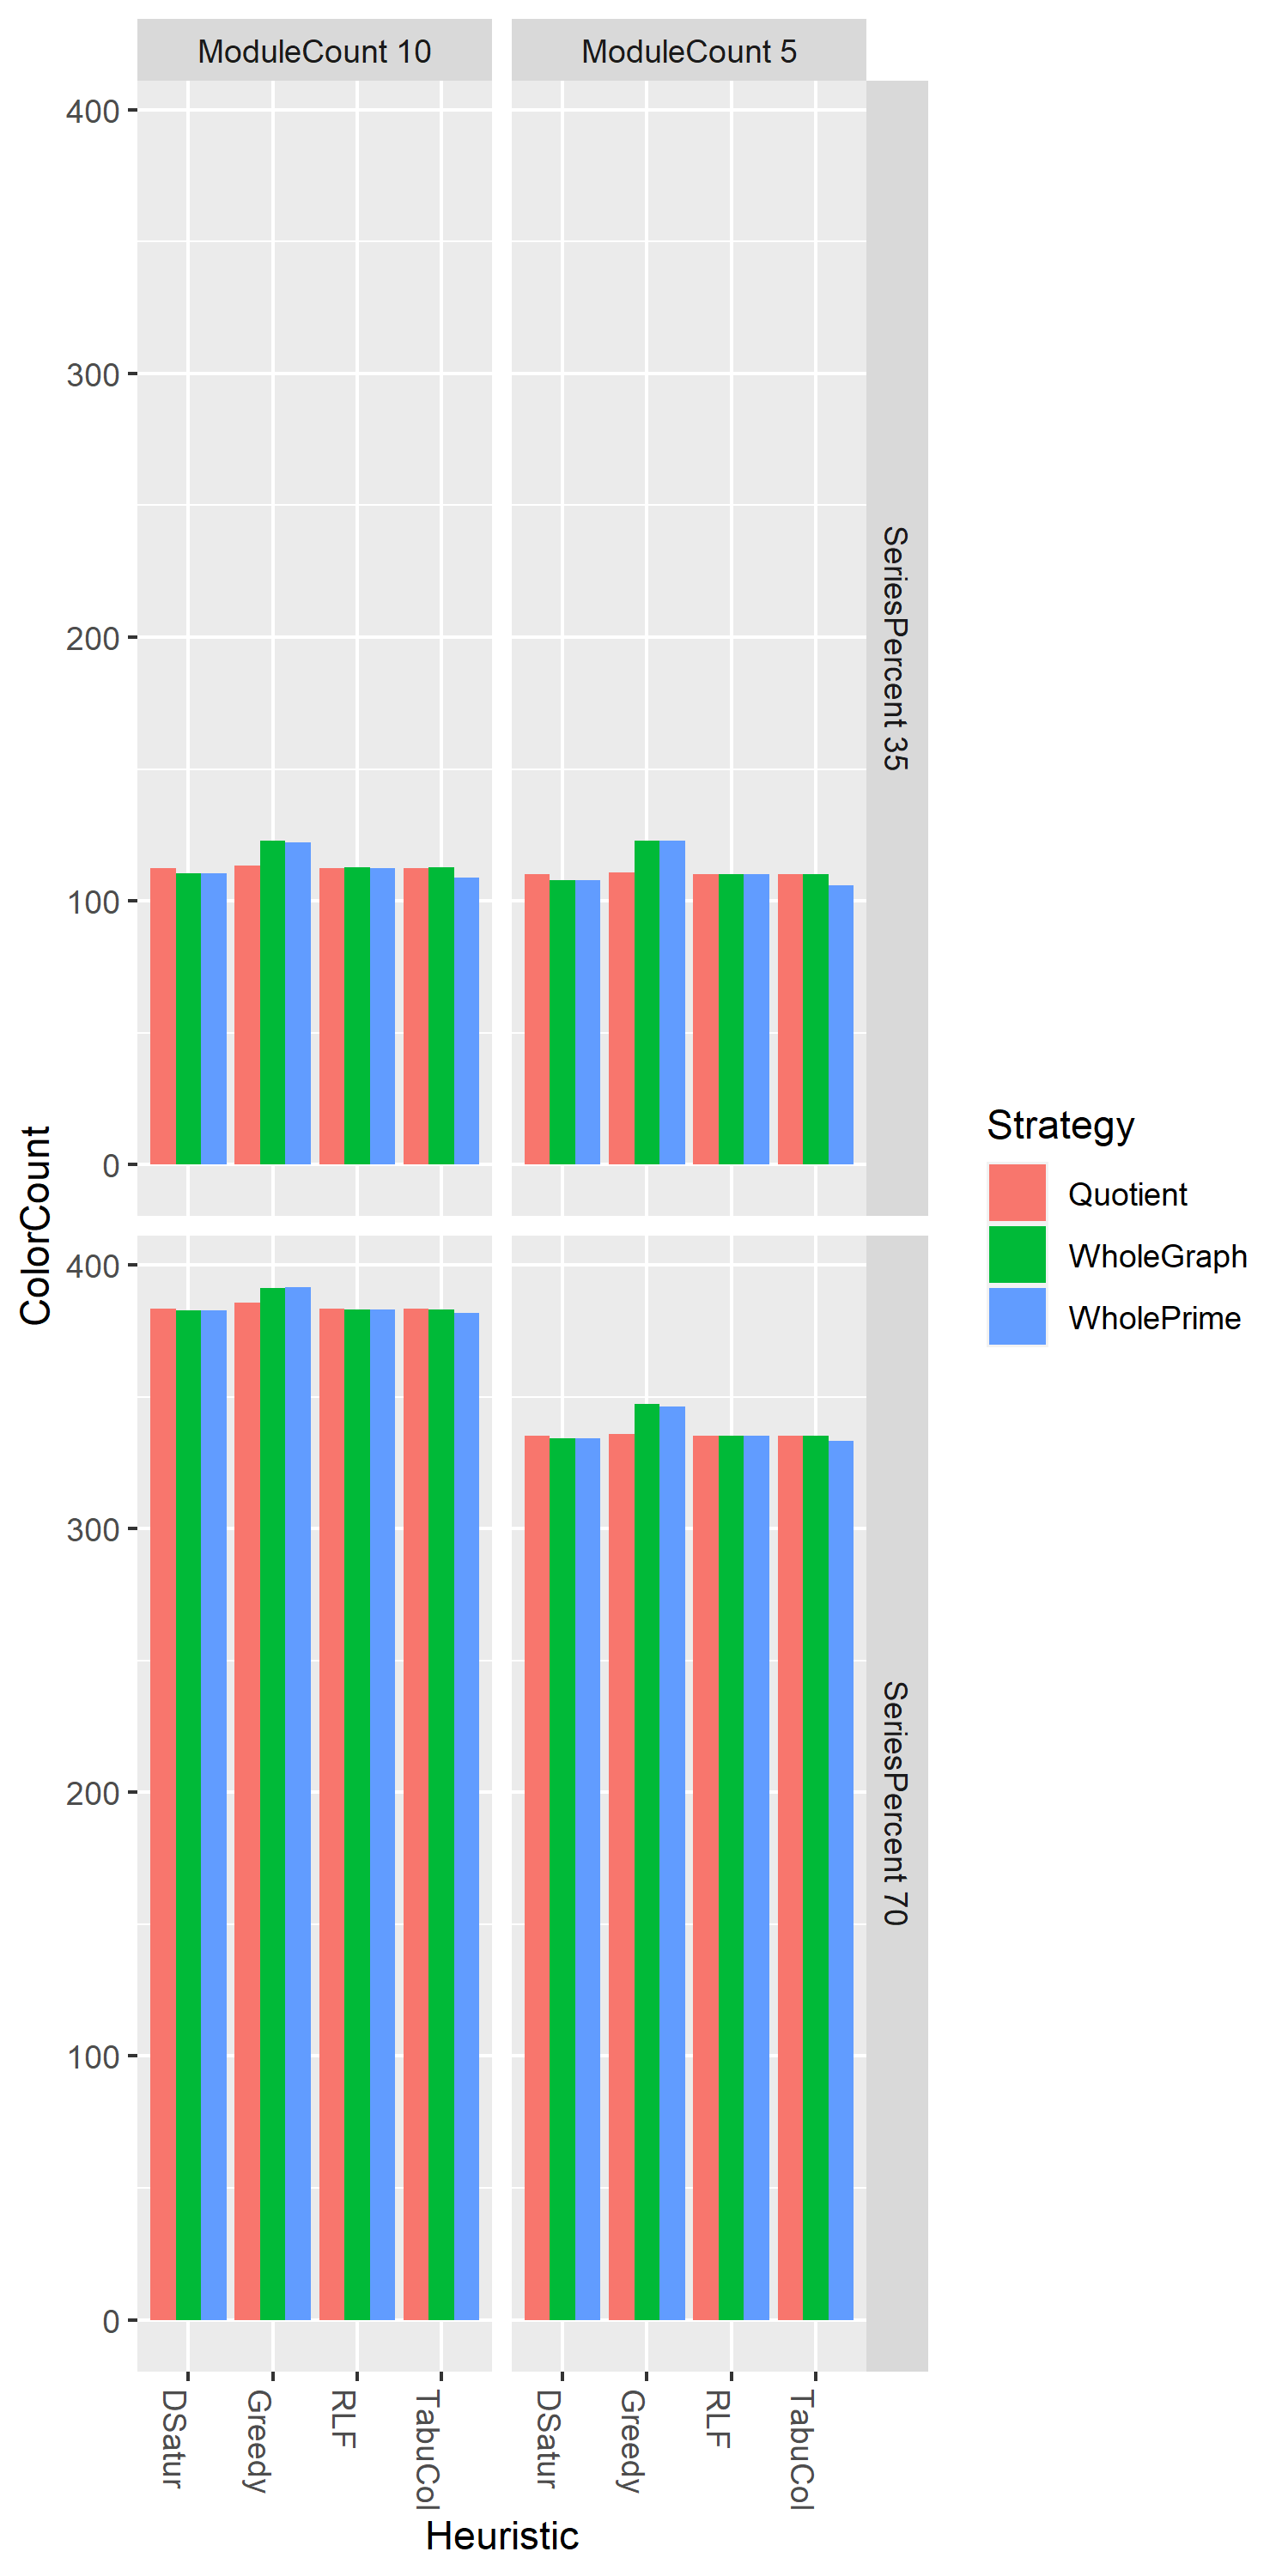
\includegraphics[width=0.9\textwidth]{Tables/1000.png}
    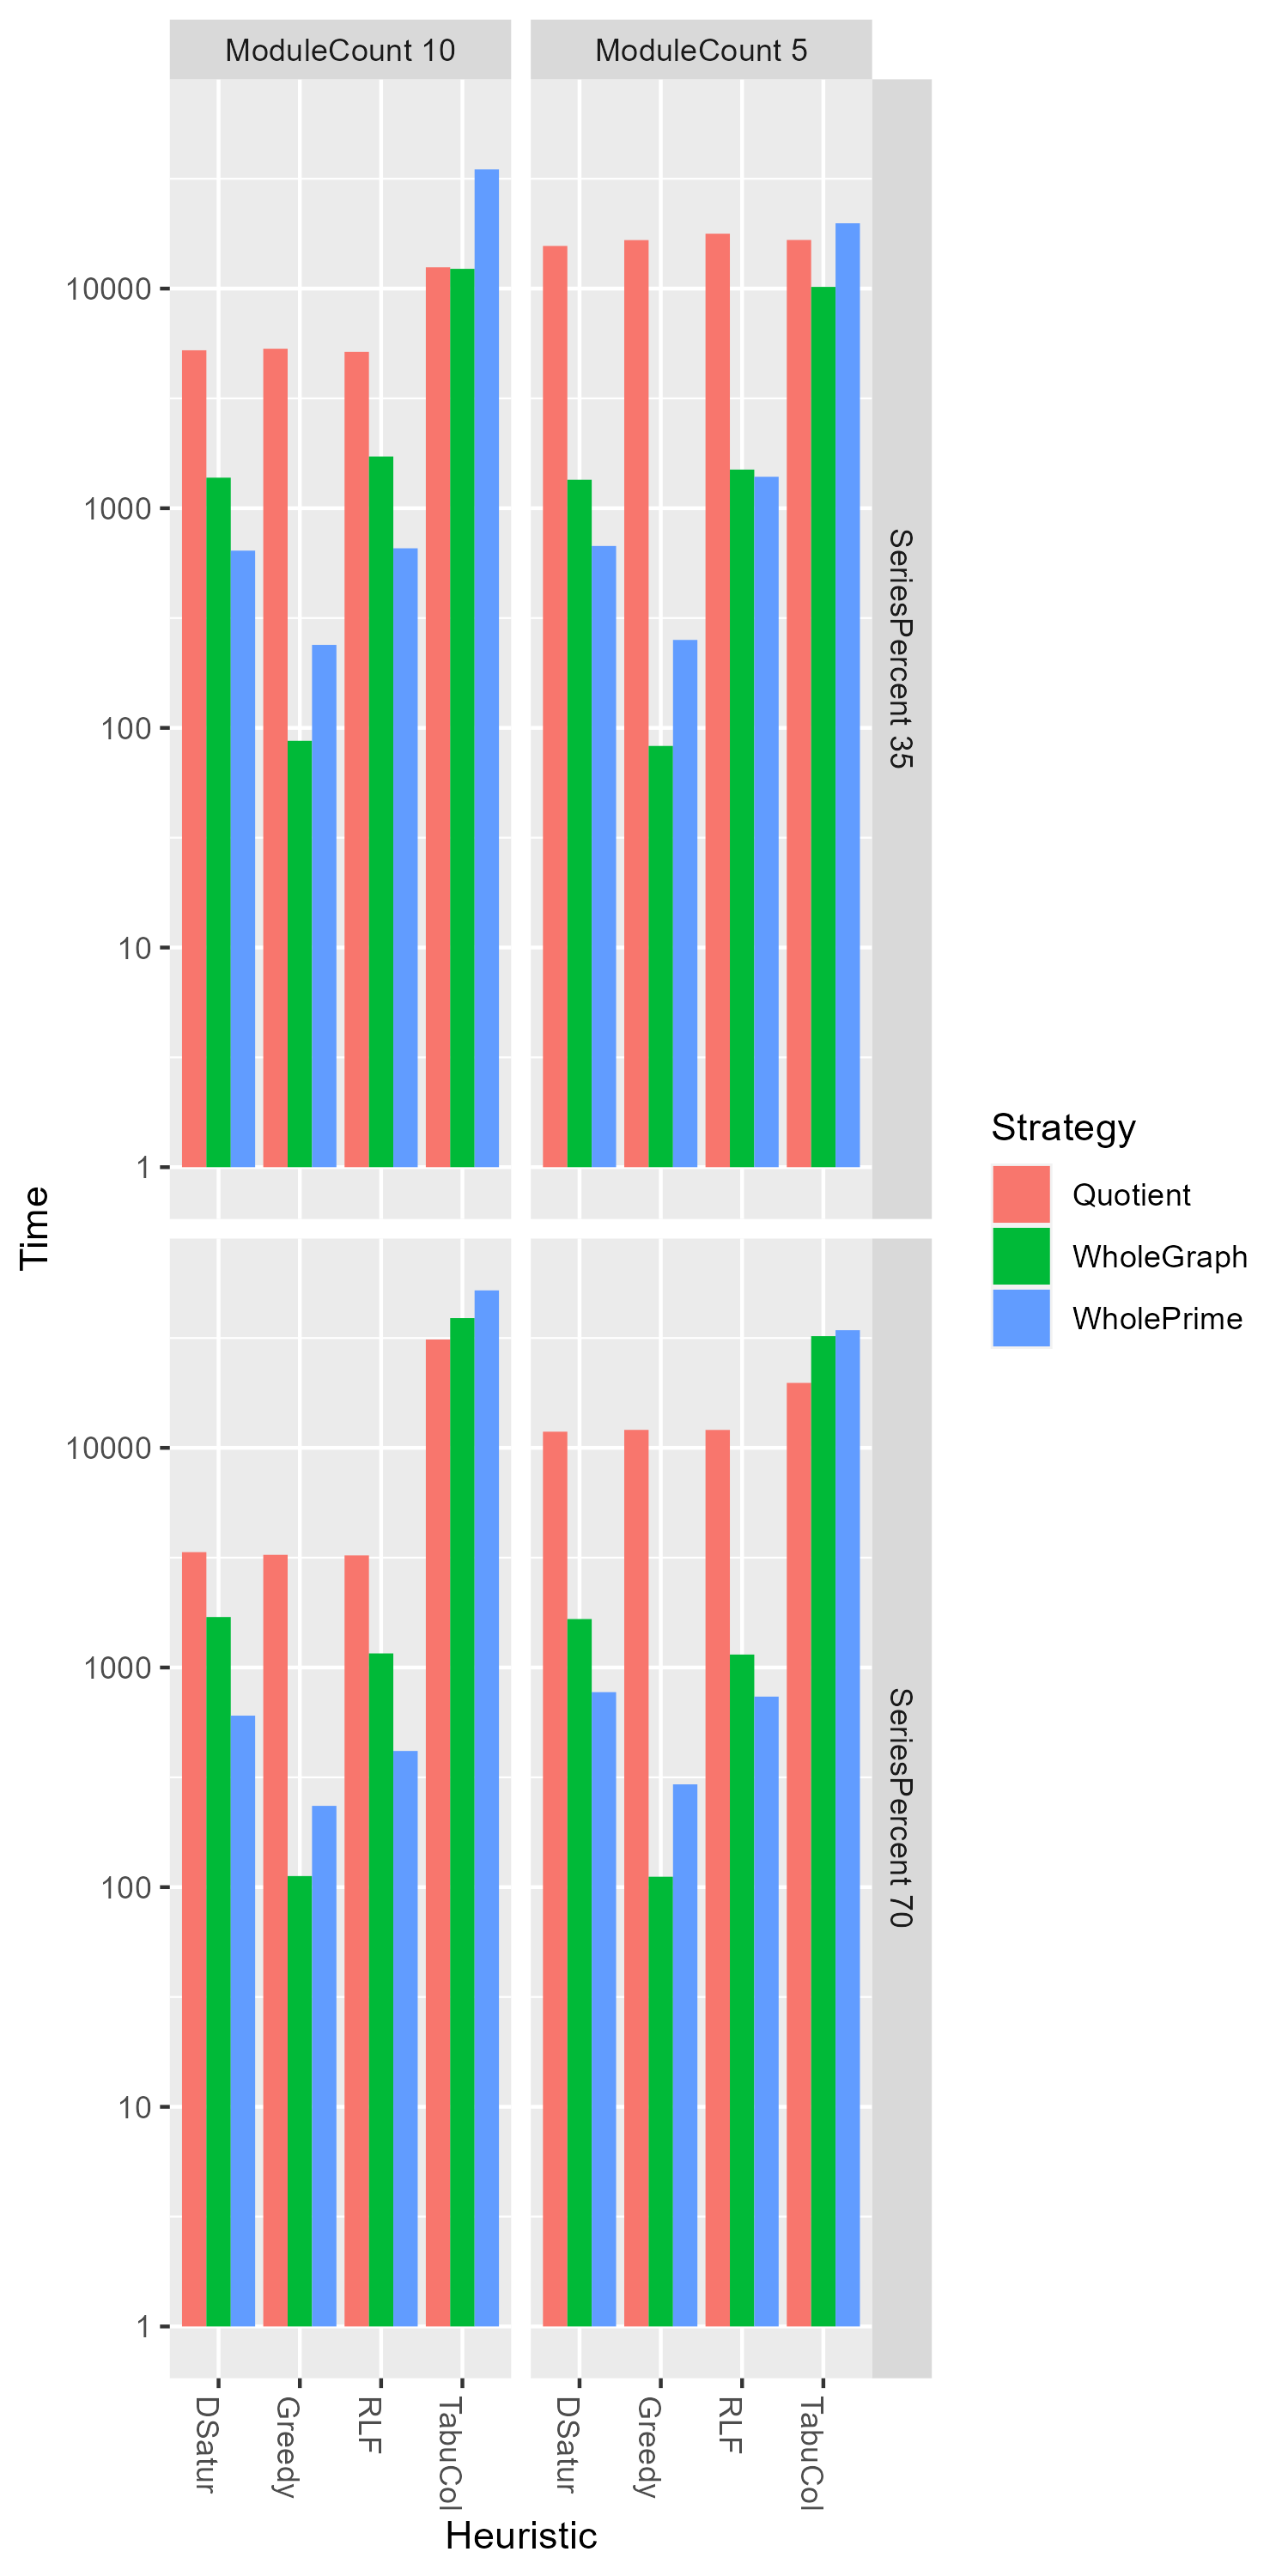
\includegraphics[width=0.9\textwidth]{Tables/1000Time.png}
    \caption{1000 verties}
\end{figure}
\begin{figure}[h]
    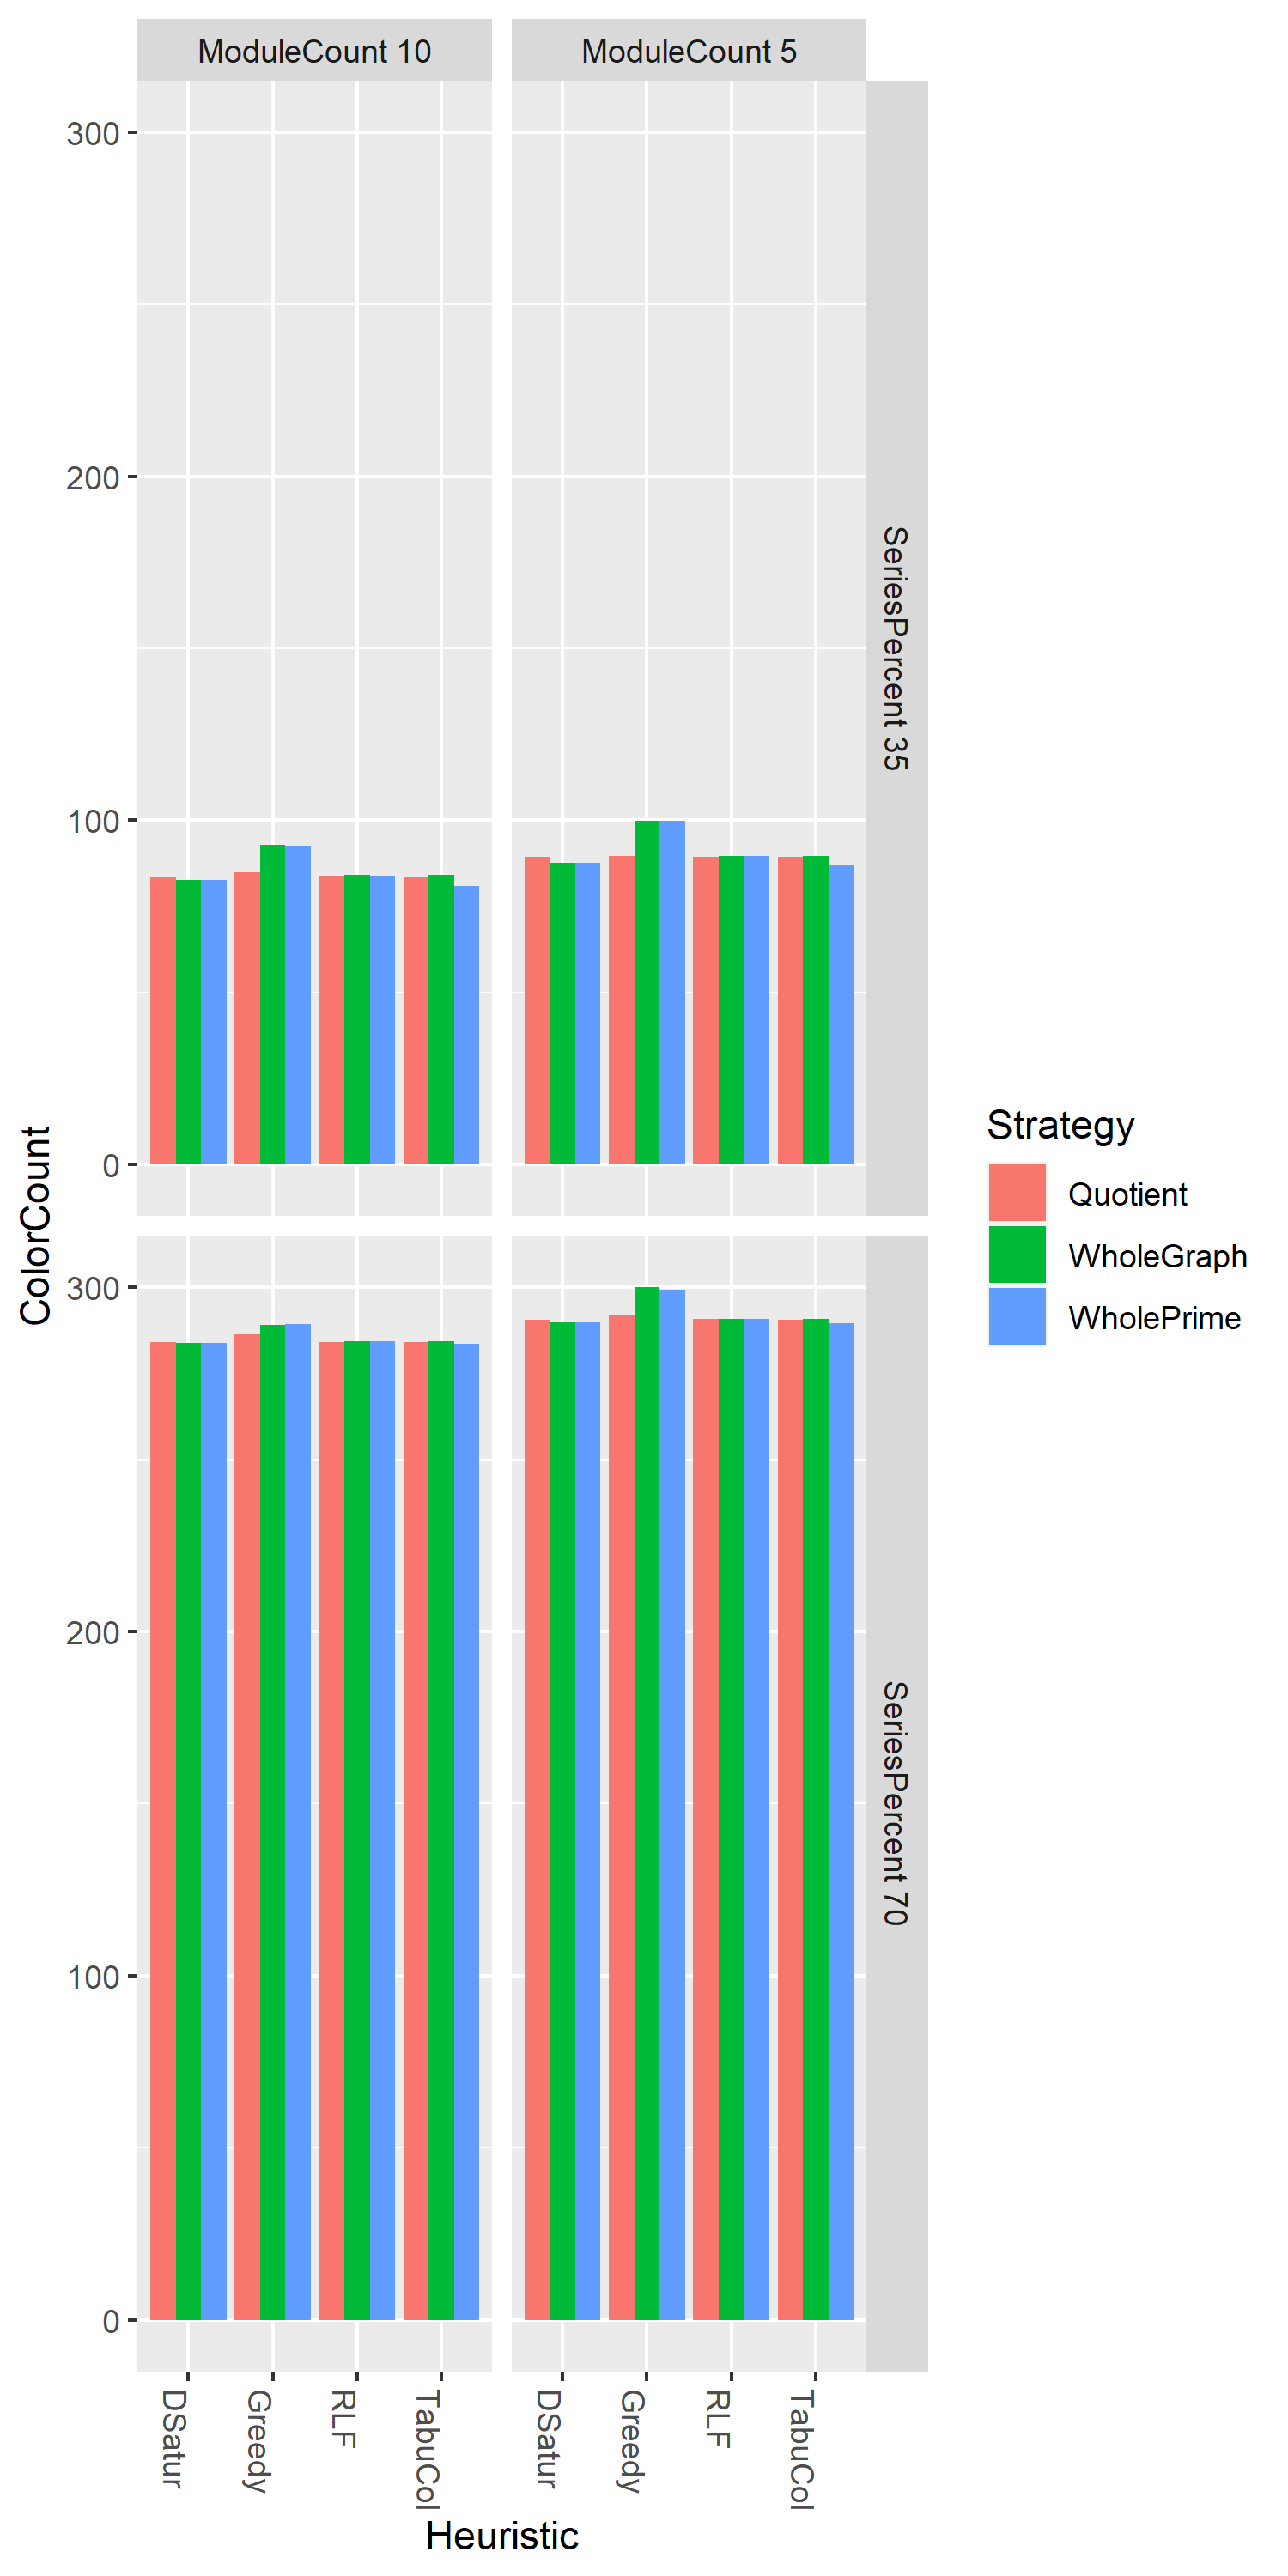
\includegraphics{Tables/750.png}
    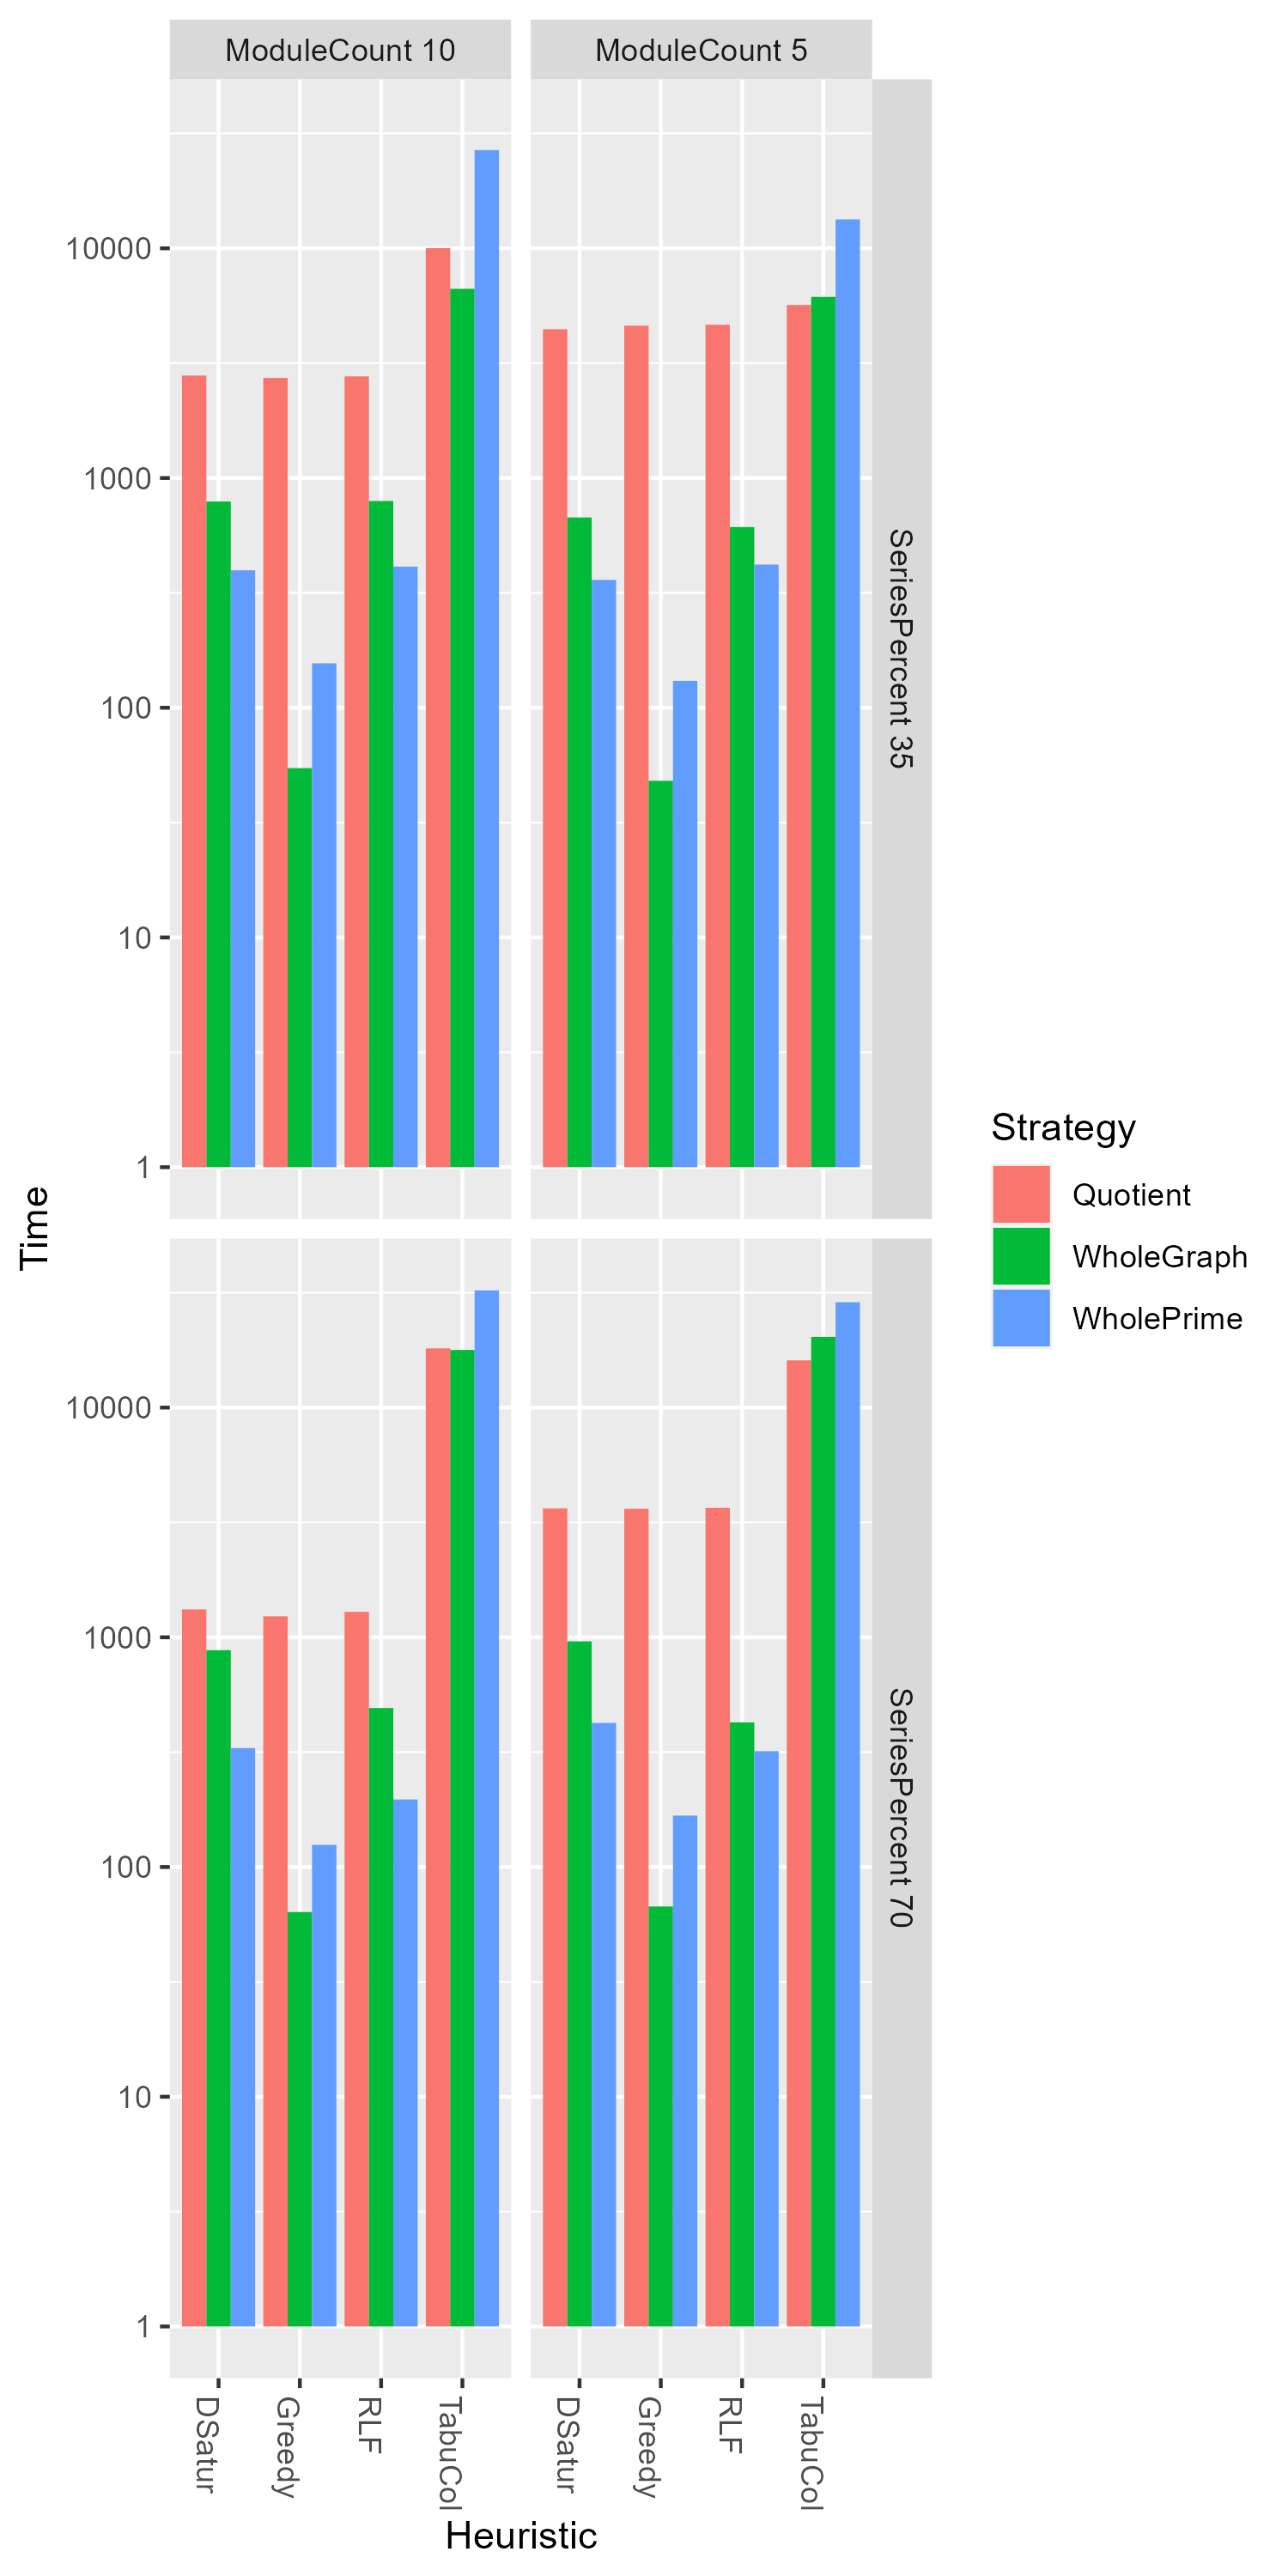
\includegraphics{Tables/750Time.png}
    \caption{750 verties}
\end{figure}
\begin{figure}[h]
    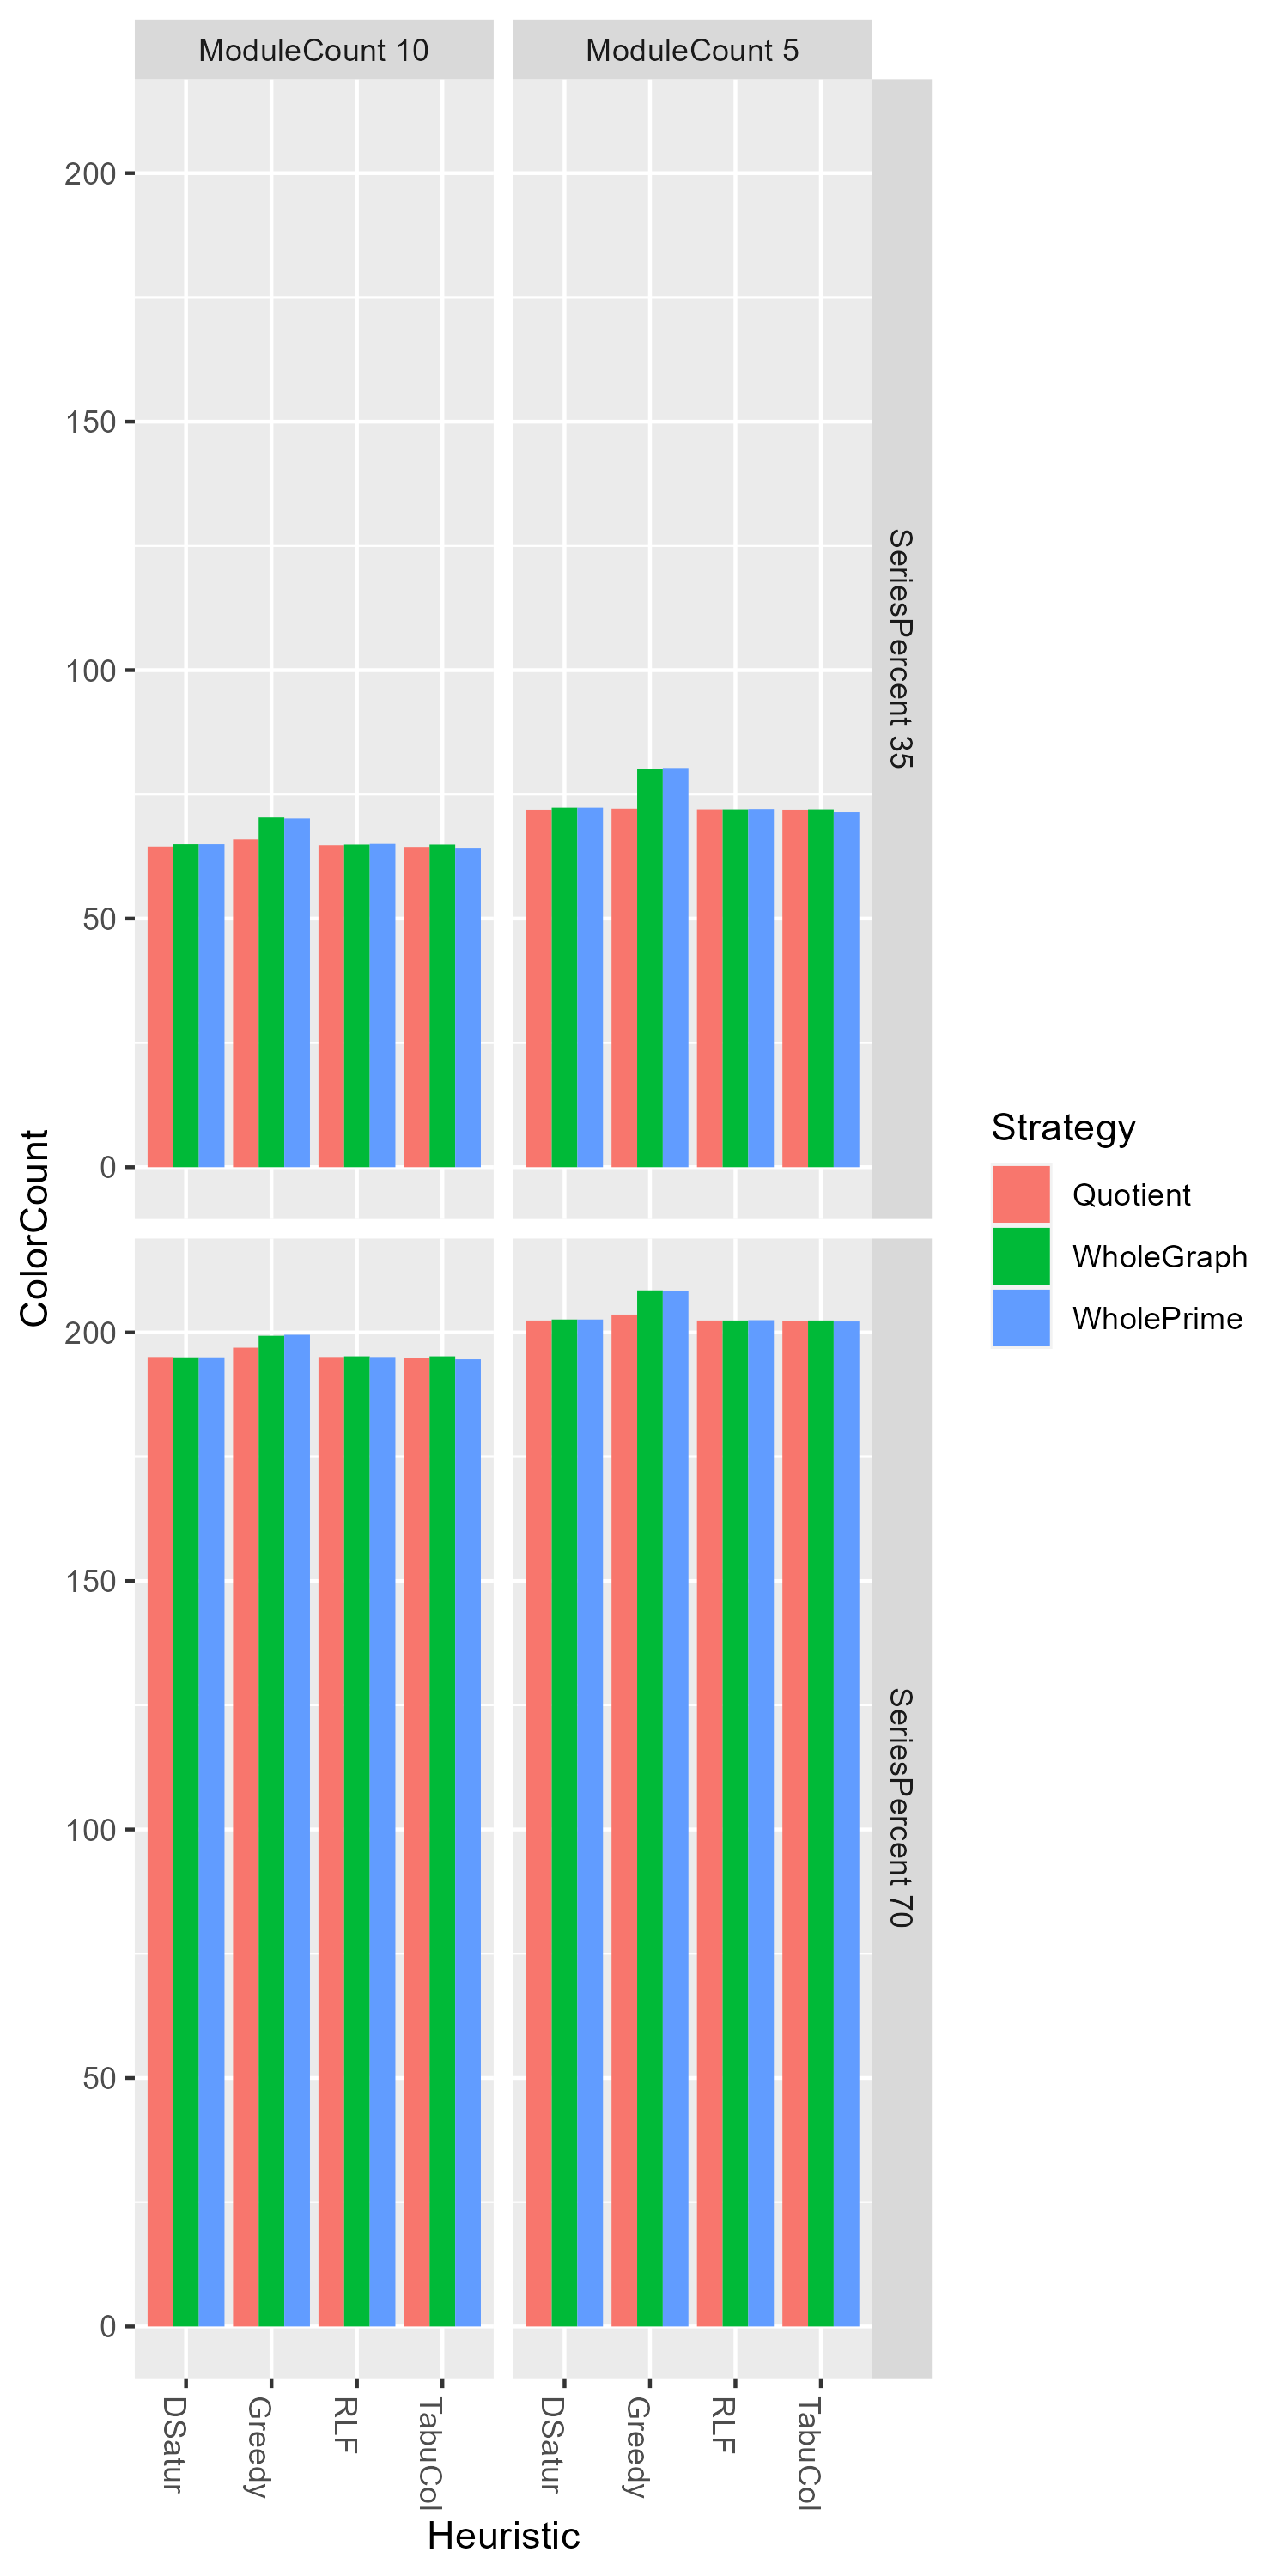
\includegraphics{Tables/500.png}
    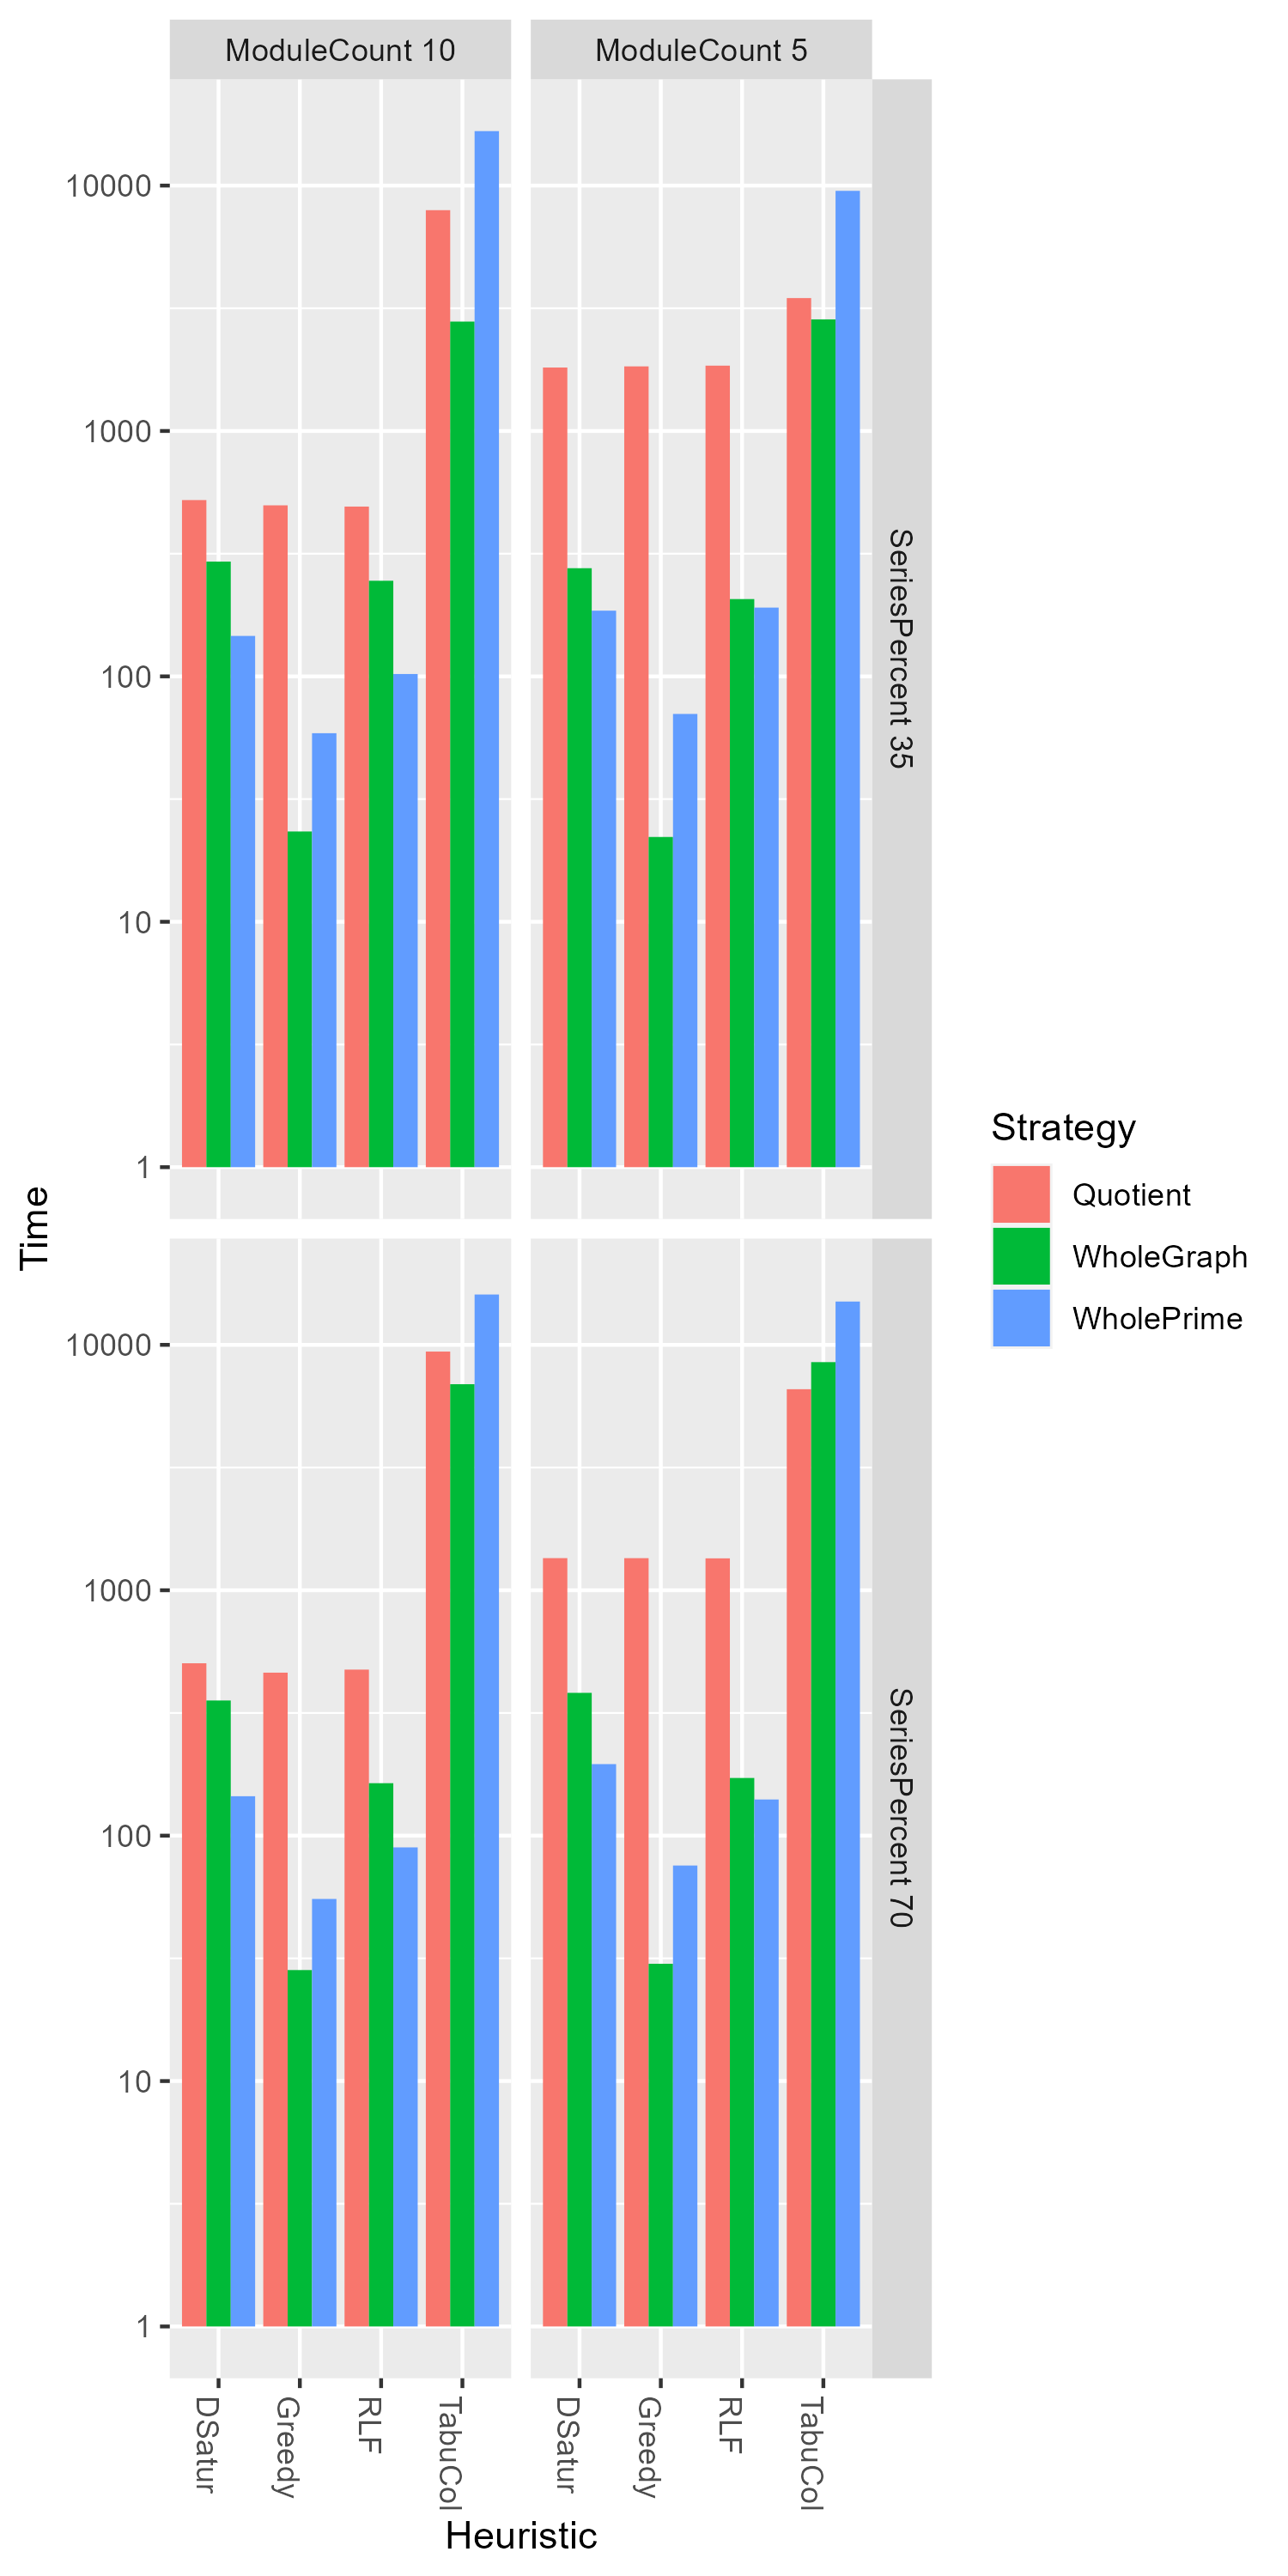
\includegraphics{Tables/500Time.png}
    \caption{500 verties}
\end{figure}
\begin{figure}[h]
    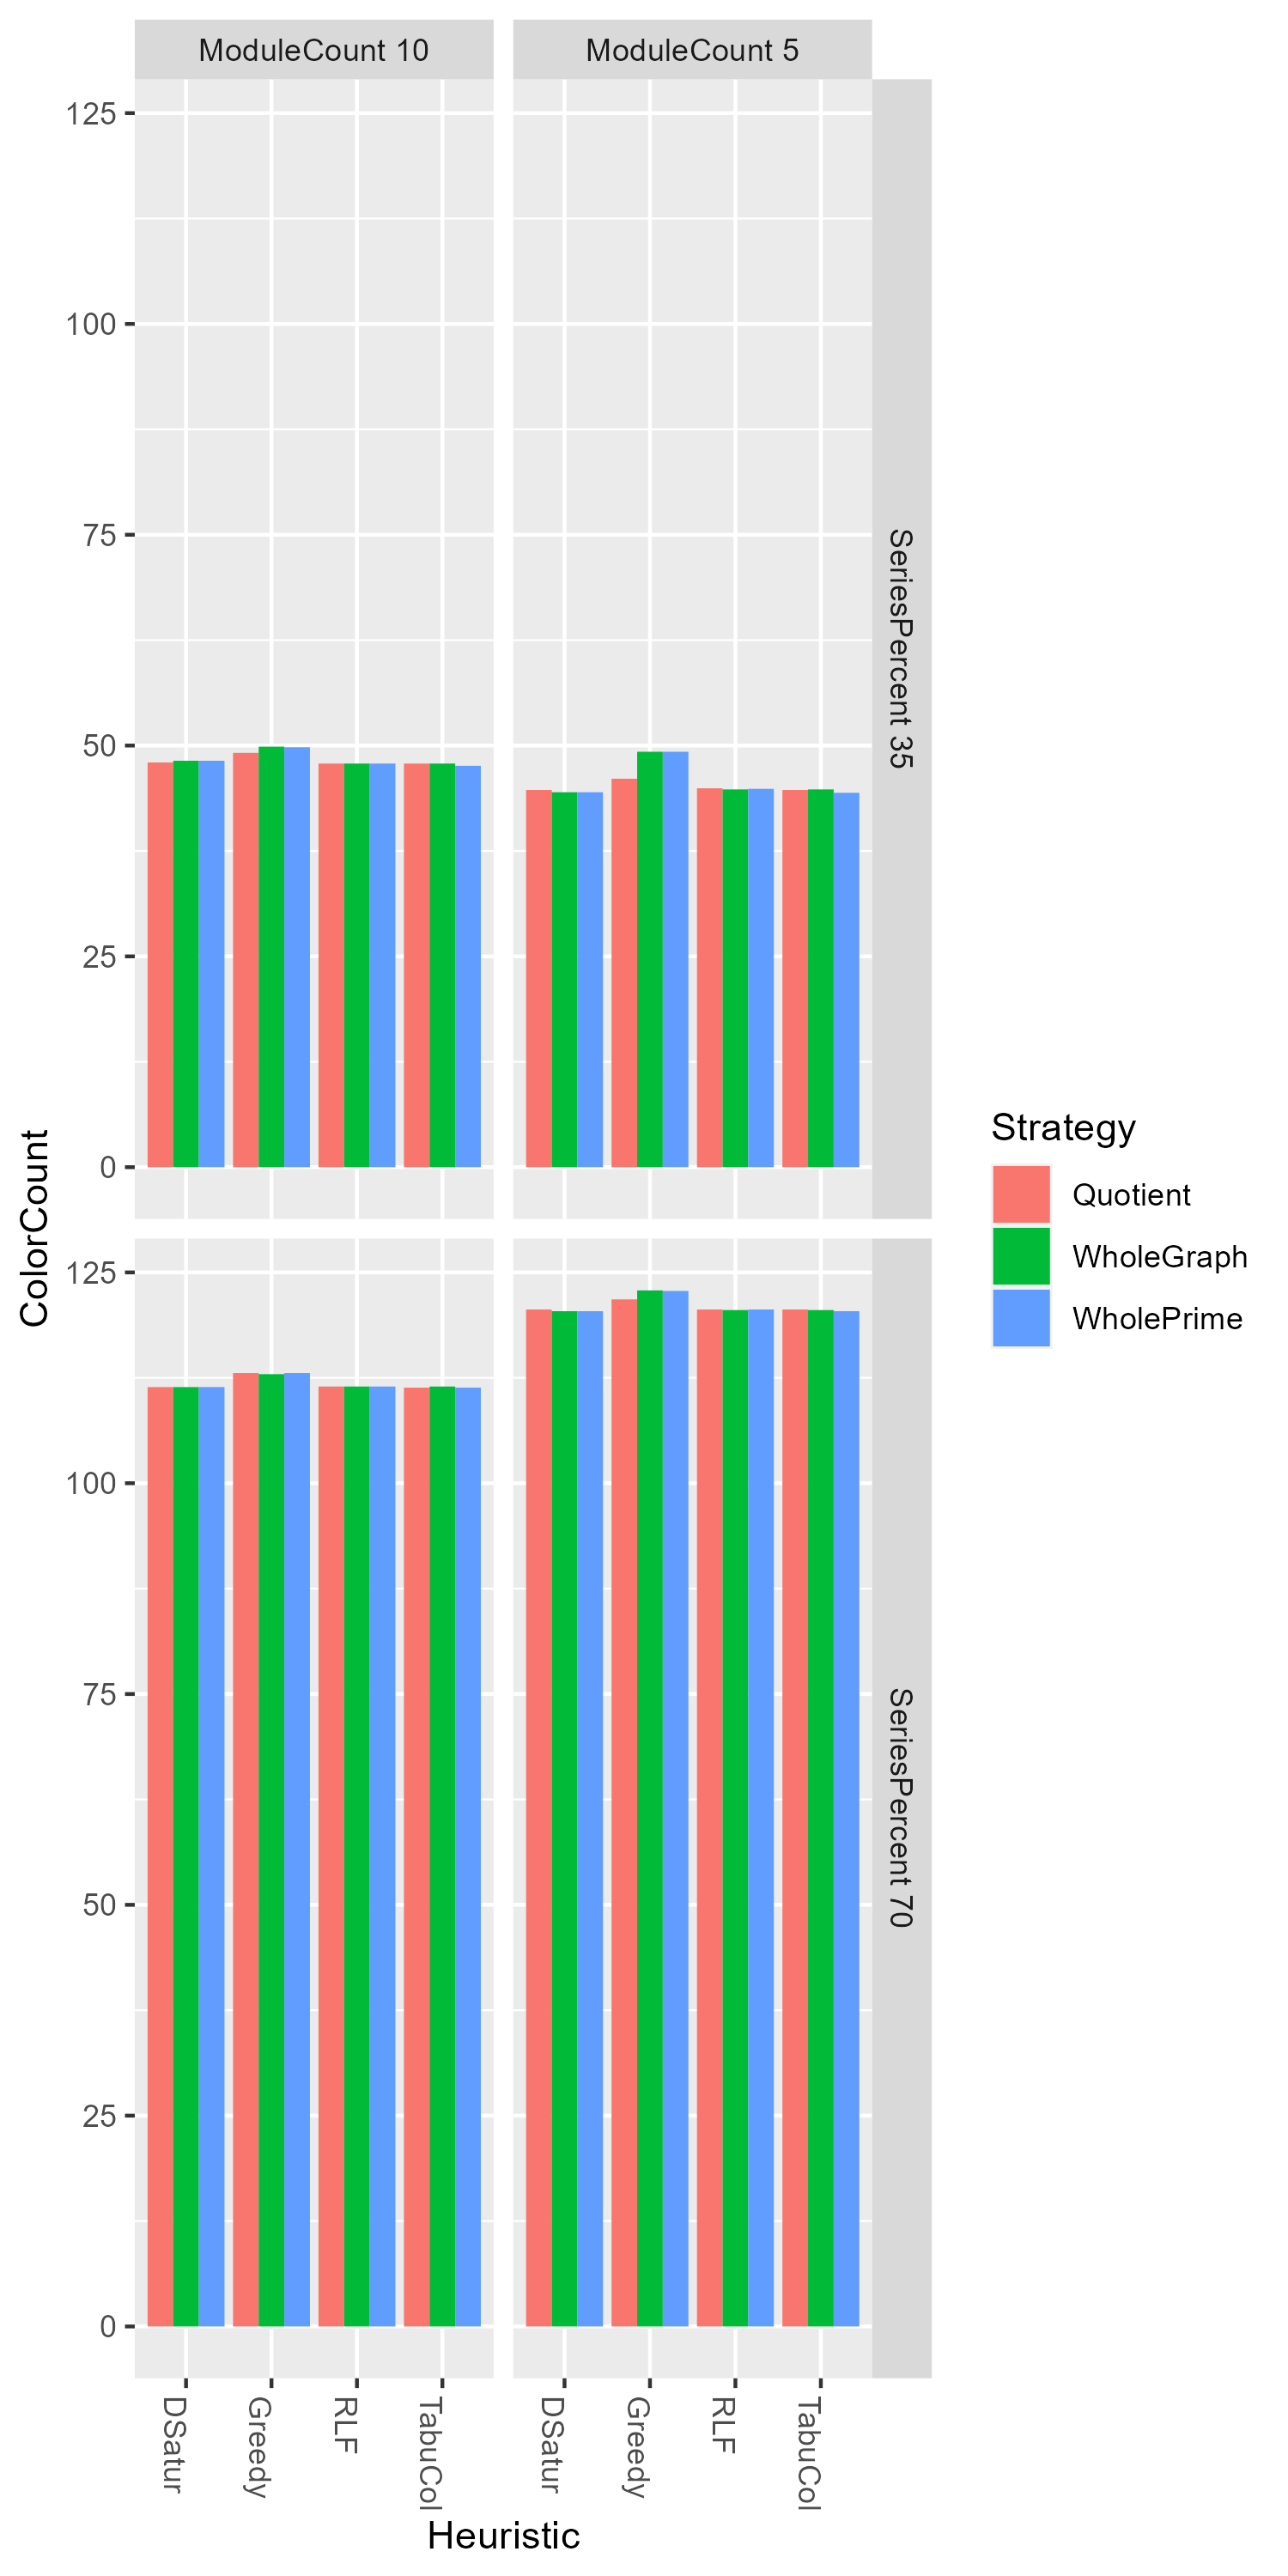
\includegraphics{Tables/250.png}
    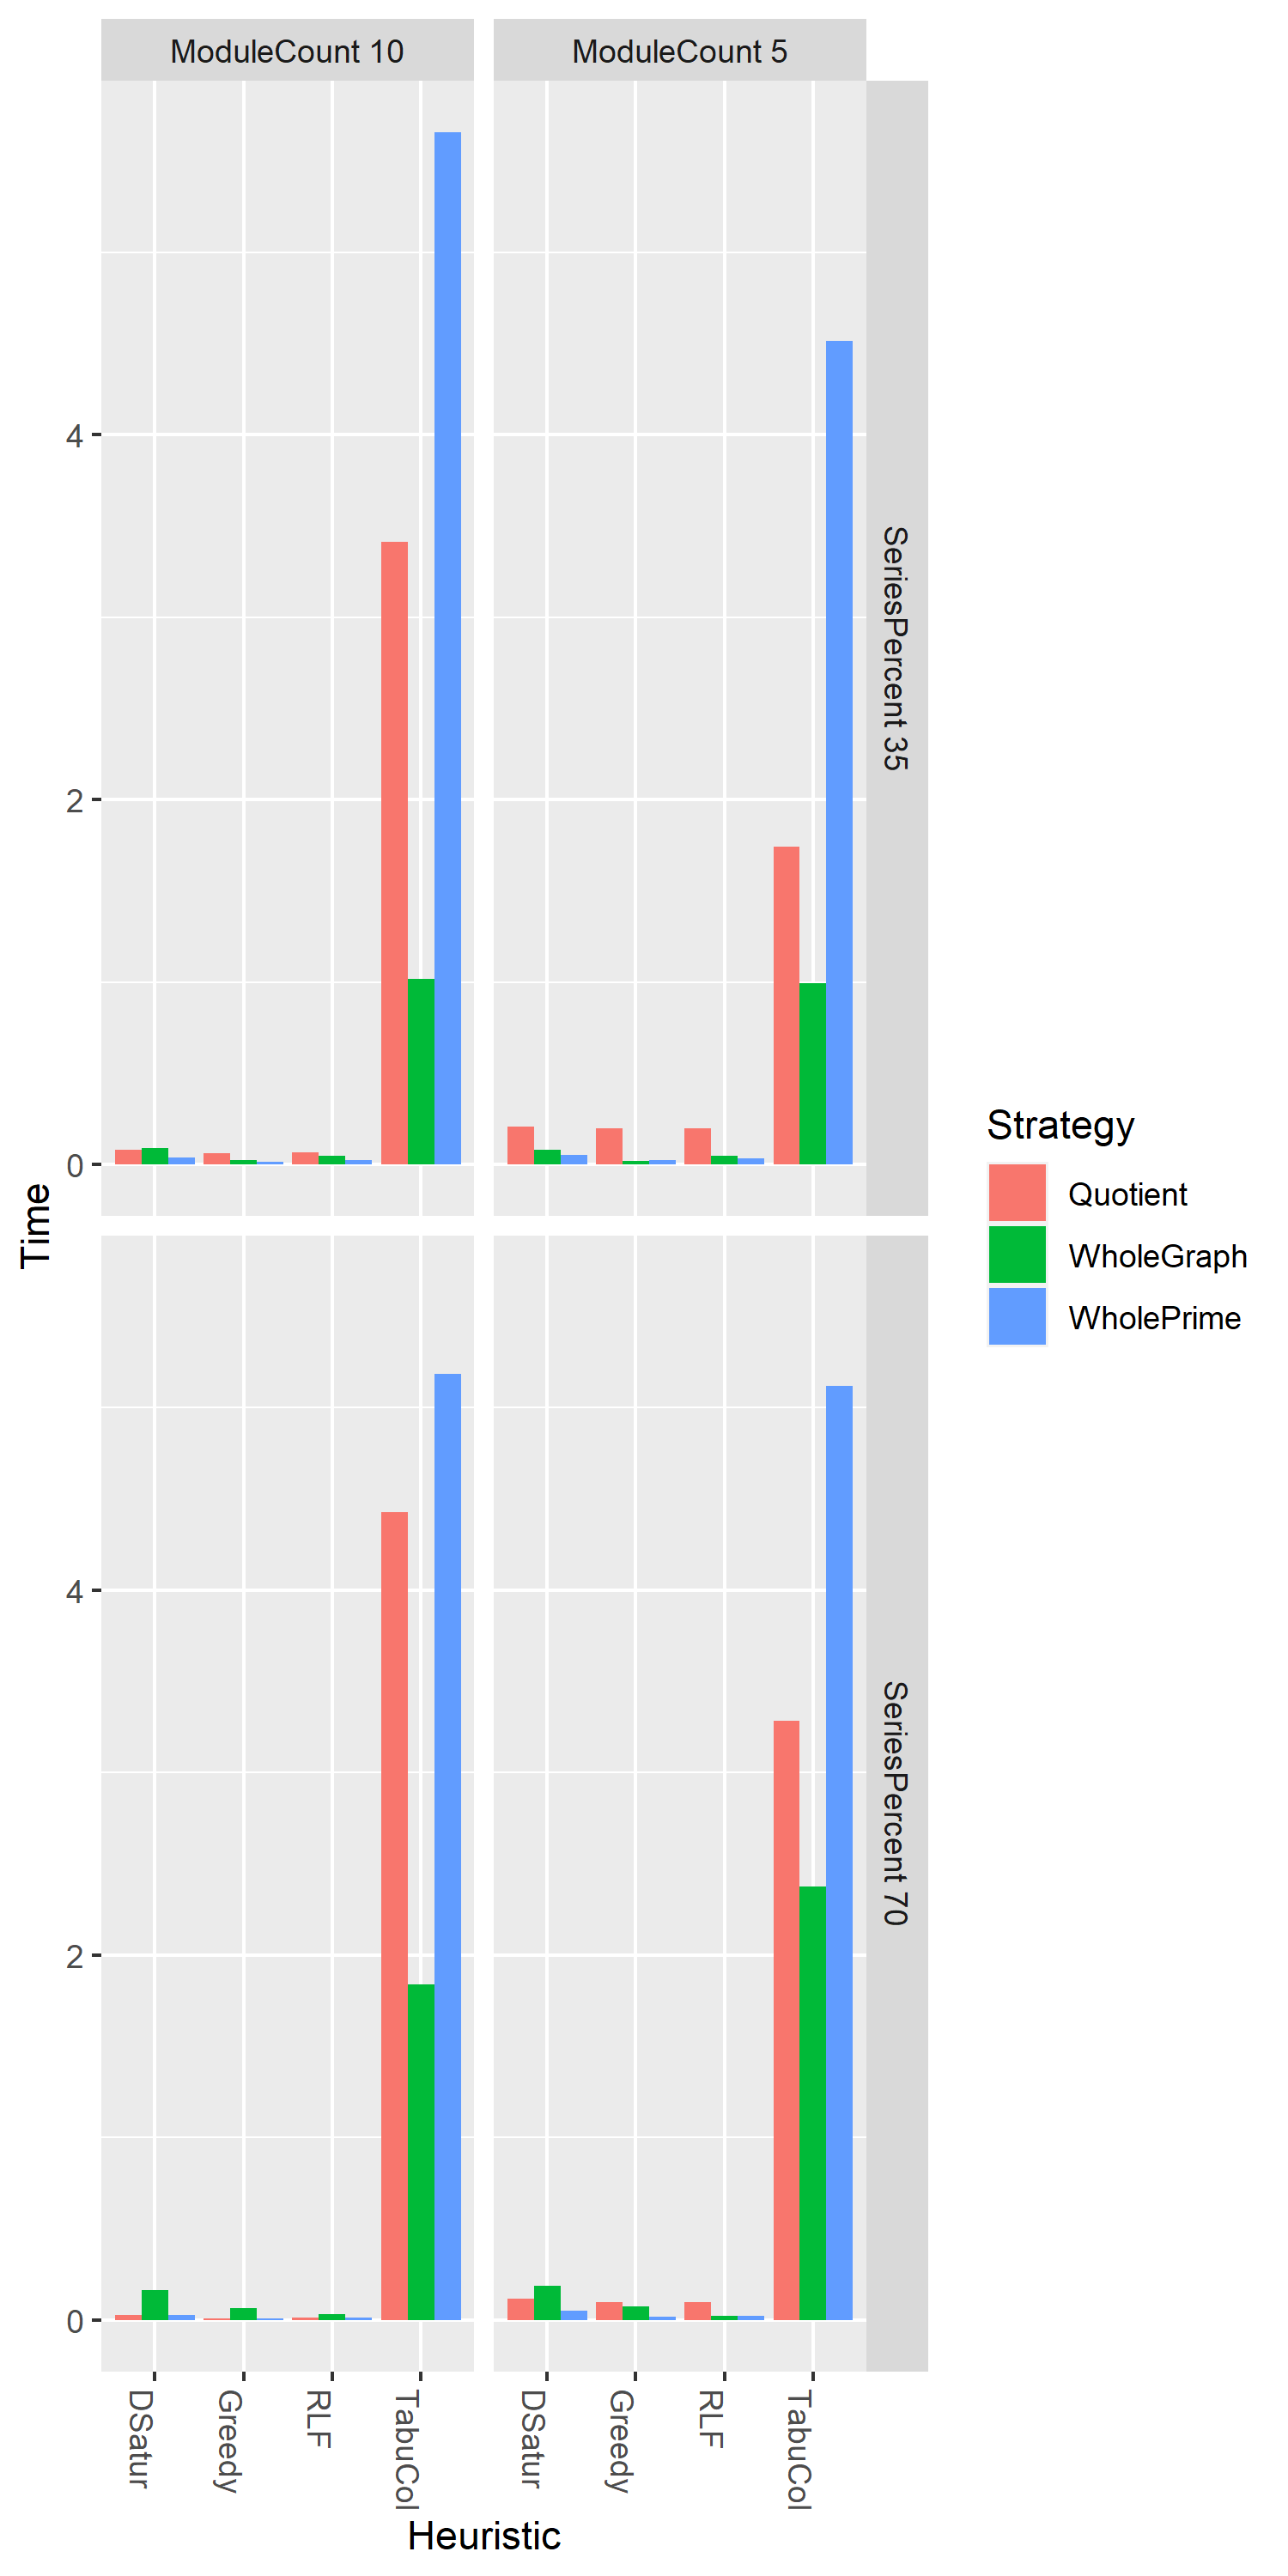
\includegraphics{Tables/250Time.png}
    \caption{250 verties}
\end{figure}

\FloatBarrier
\subsection{Discussion}

Something that we can see from the tables, most easily from
\autoref{table:combined}, is that applying a heuristic locally on prime modules
doesn't significantly affect the resulting color for RLF,Greedy and DSatur. It
does however seem to give a minor improvement for TabuCol. In situations where
one would consider using TabuCol with it's comparably larger execution time in
the first place, so could it be reasonable to use the modular decomposition for
increased performance.

Looking at the difference between series probability of 35\% versus 70\%, it
seems like the performance for TabuCol is better for the sparser graph with
35\% series probability. There also doesn't seem to be any direct difference
with the number of prime modules, both 10 and 5 seem to perform similarly.

The result for the quotient strategy always seems comparable to the performance
of RLF. While it can be seen to outperform pure RLF very slightly for some combinations,
such as \autoref{table:quotient}, 
\todo{More tests to ensure significance? Redundant as it's still an arbitrary test set?}
so is the sample size to small to draw any conclusions. 
It also exhibits a much larger runtime, most notable for the DIMACS test set.
The potential performance benefit most likely doesn't compensate for the
increased runtime however, even with a more optimized implementation.


Looking at the time taken to color the graphs, we can see that the modular decomposition might have a 
use in decreasing the execution time. Graph coloring algorithms with execution time that
doesn't scale linearly with the size of the graph could benefit from being applied
more times on smaller subgraphs. But whether or not this is worth it in practice 
depends on the ability to implement the modular decomposition tree in linear time, 
and if the added computations can be compensated by large enough graphs.

Another possible advantage with the modular decomposition is that it could
allow for more easily implemented parallelised coloring algorithms. As the
modular decomposition tree creates a partition of the graph vertices, so can
the different parts of the modular decomposition tree be colored in parallel,
which could compensate for the increased runtime when for example using TabuCol.

\printbibliography

\newpage
\Baksida %Kommentera för att bli av med loggan
\vspace*{13cm}
%Kandidatuppsats 2010:11\\ %Fyll i löpnummer
Datalogi\\
%September 2010\\\\ % Fyll i månad och år
\monthyeardate\today\\
www.math.su.se\\\\
Beräkningsmatematik\\
Matematiska institutionen\\
Stockholms universitet\\
106 91 Stockholm\\

\end{document}
